\documentclass[12pt]{report}
\usepackage[utf8]{inputenc}
\usepackage[english]{babel}
\usepackage[letterpaper, portrait, margin=1in]{geometry}
\usepackage{amsmath}
\numberwithin{equation}{section}
\usepackage{amssymb}
\usepackage{graphicx}
\usepackage{parskip}
\usepackage{xcolor}
\usepackage{physics}
\usepackage{empheq}
\usepackage{cancel}
\usepackage{hyperref}
\hypersetup{colorlinks = true, urlcolor = blue, linkcolor = red, citecolor = red}
\usepackage{enumerate}
\usepackage{tikz}
\usepackage{float}
\usepackage{tcolorbox}
\usepackage{booktabs}
\usepackage[bottom]{footmisc}

\def\rcurs{{\mbox{$\resizebox{.08in}{.08in}{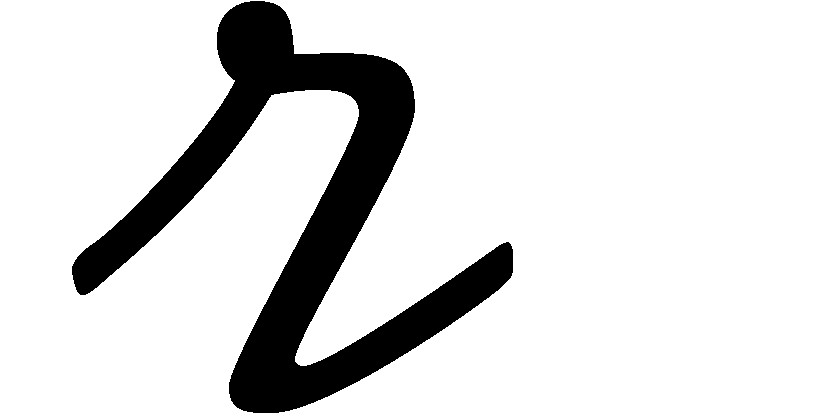
\includegraphics{scriptr/ScriptR}}$}}}
\def\brcurs{{\mbox{$\resizebox{.08in}{.08in}{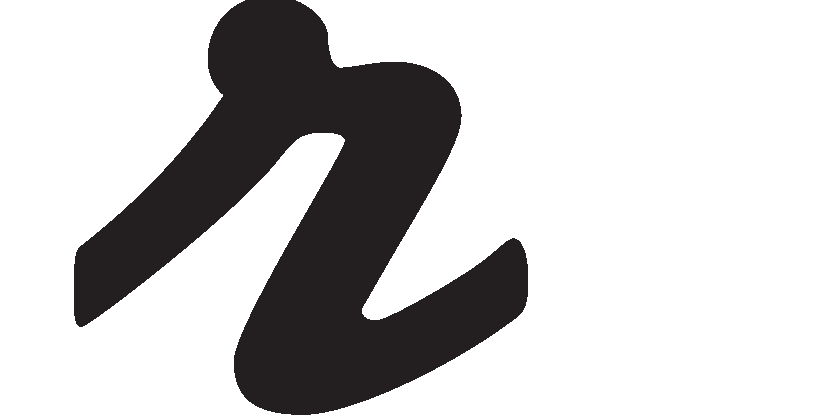
\includegraphics{scriptr/BoldR}}$}}}
\def\hrcurs{{\mbox{$\hat \brcurs$}}}

\def\p{{\mbox{$\boldsymbol{\mathrm{p}}$}}}
\def\f{{\mbox{$\boldsymbol{\mathrm{f}}$}}}
\def\P{{\mbox{$\boldsymbol{\mathrm{P}}$}}}
\def\M{{\mbox{$\boldsymbol{\mathrm{M}}$}}}
\def\E{{\mbox{$\boldsymbol{E}$}}}
\def\D{{\mbox{$\boldsymbol{D}$}}}
\def\B{{\mbox{$\boldsymbol{B}$}}}
\def\H{{\mbox{$\boldsymbol{H}$}}}
\newcommand{\unit}[1]{\hat{\boldsymbol{#1}}}
\newcommand{\bd}[1]{\boldsymbol{#1}}
\renewcommand{\b}[1]{\boldsymbol{#1}}
\renewcommand{\vec}[1]{\boldsymbol{#1}}

\definecolor{dmb}{HTML}{003366}

\begin{document}
	
	\title{\textbf{Electrodynamics: A Brief Overview\\\normalsize From \textit{Introduction to Electrodynamics} by David J. Griffiths}}
	\author{\textbf{Yi J. Zhu}}
	\date{August 24, 2020\\\vspace{1em}\small Updated \today}
	\maketitle
	\thispagestyle{empty}
	
	\tableofcontents
	
	\chapter{Electrostatics}
	
	Electrostatics concerns the properties associated with a static distribution of charges. The results in this section follow from Coulomb's Law, which states that the force of a test charge $ q $ due to a single point charge $ Q $ is given by,
	\begin{equation}
		\b{F} = \frac{1}{4\pi\epsilon_0}\frac{Qq}{\rcurs^2}\hrcurs
	\end{equation}
	
	\section{Electrostatic Field}
	
	 The electric field for a collection of point charges is defined\footnote{This results from Coulomb's law and the principle of superposition.},
	\begin{equation}
		\boldsymbol{E}(\boldsymbol{r}) = \frac{1}{4\pi\epsilon_0}\sum_i \frac{q_i}{\rcurs_i^2}\hat{\brcurs}_i
	\end{equation}
	Generalizing for a continuous charge distribution,
	\begin{equation}
		\boxed{\boldsymbol{E}(\boldsymbol{r}) = \frac{1}{4\pi\epsilon_0}\int_V \frac{\rho(\boldsymbol{r}')}{\rcurs^2}\hat{\brcurs}\,d\tau'}
	\end{equation}
		
	We define the electric field because we can then express the force on a test charge $ q $ as,
	\begin{equation}
		\boxed{\b{F} = q\E}
	\end{equation}
	This is much more convenient than applying Coulomb's law directly because we need only determine the electric field of a charge configuration once to understand the behavior of \textit{any} test charge at \textit{any} location. 
	
	We can view the electric field (and fields in general) as simply a bookkeeping term. However, it is often more useful useful to think of $ \E $ as a physical ``thing."
	
	\subsection{Divergence of an Electrostatic Field}
	Let's now calculate the divergence of $ \boldsymbol{E} $\footnote{Notice that the derivative is with respect to $ \boldsymbol{r} $ but the integral is with respect to $ \boldsymbol{r}' $.},
	\begin{align}
		\div\boldsymbol{E} &= \div \left(\frac{1}{4\pi\epsilon_0}\int_V \frac{\rho(\boldsymbol{r}')}{\rcurs^2}\hat{\brcurs}\,d\tau'\right)\\
		&= \frac{1}{4\pi\epsilon_0} \int_V \div \left(\frac{\rho(\boldsymbol{r}')}{\rcurs^2}\hat{\brcurs}\right)\,d\tau' \\
		&= \frac{1}{4\pi\epsilon_0} \int_V \div \left(\frac{\boldsymbol{\hat{\brcurs}}}{\rcurs^2}\right)\rho(\boldsymbol{r}')\,d\tau' \\
		&= \frac{1}{4\pi\epsilon_0} \int_V \left(4\pi\ \delta(\brcurs)\right)\rho(\boldsymbol{r}')\,d\tau' \\
		&= \frac{1}{4\pi\epsilon_0} \left(4\pi\ \rho(\boldsymbol{r})\right) 
	\end{align}
	\begin{equation}
		\boxed{\div\boldsymbol{E} = \frac{1}{\epsilon_0}\rho(\boldsymbol{r})}
	\end{equation}
	
	Applying the Divergence Theorem,
	\begin{equation}
		\oint_S \boldsymbol{E}\cdot d\boldsymbol{a} = \int_V \div \boldsymbol{E}= \int_V \frac{\rho(\boldsymbol{r})}{\epsilon_0} = \frac{Q_\text{enc}}{\epsilon_0}
	\end{equation}
	where $ Q_\text{enc} $ is the charge enclosed in the Gaussian surface. This is known as Gauss's Law\footnote{Dunno why it's not ``Gauss' Law."},
	\begin{equation}
		\boxed{\oint_S \boldsymbol{E}\cdot d\boldsymbol{a} =\frac{Q_\text{enc}}{\epsilon_0}}
	\end{equation}
	As Griffiths astutely states: Gauss's law is always \textit{true}, but it is not always \textit{useful}.

	\subsection{Curl of an Electrostatic Field}
	In studying the curl of a general electrostatic field, we can first examine the curl of a point charge. At a glance, the curl of such a field must be zero. We can prove this via Stokes Theorem by showing that the line integral of $ \boldsymbol{E} $ for an closed curve is zero,
	\begin{align}
		\int_{\boldsymbol{a}}^{\boldsymbol{b}} \boldsymbol{E}\cdot d\boldsymbol{l} & =\int_{\boldsymbol{a}}^{\boldsymbol{b}} \left( \frac{q}{4\pi\epsilon_0\ r^2}\ \boldsymbol{\hat{r}}\right) \cdot \left(dr\ \boldsymbol{\hat{r}} + r\ d\theta\ \boldsymbol{\hat{\theta}} + r\sin\theta\ d\phi\ \boldsymbol{\hat{\phi}}\right)\\
		&= \frac{q}{4\pi\epsilon_0}\int_{r_a}^{r_b} \frac{dr}{r^2} = \frac{q}{4\pi\epsilon_0} \left(\frac{1}{r_a} - \frac{1}{r_b}\right) = 0 \quad\text{when }r_a=r_b
	\end{align}
	Now we have only shown that a point charge has no curl. However, all electrostatic fields can be formed by a superposition of point charges and curl is a linear operator. Thus, for all electrostatic fields,
	\begin{equation}
		\boxed{\curl \boldsymbol{E} = 0}
	\end{equation}
	
	\section{Electric Potential}
	
	The curl of an electrostatic field is zero so by Stokes' Theorem  the field is conservative\footnote{Recall conservative means that the line integral is path-independent.}\textsuperscript{,}\footnote{A simple proof: imagine points $ a $ and $ b $ are connected via two distinct curves, $ C_1 $ and $ C_2 $. Then, $ \oint_{a\to b}\boldsymbol{E}\cdot d\boldsymbol{l}$ via $ C_1 $ plus $ \oint_{b\to a}\boldsymbol{E}\cdot d\boldsymbol{l}$ via $ C_2 $ equals zero because $ a\to b\to a $ is a closed curve---so by Stokes' Theorem, the loop integral of a irrotational field is zero. Thus, the line integral along both curves must be the same and, in general, the integral is path-independent.}. Furthermore, we can define a scalar potential for a conservative vector field such that,
	\begin{equation}
		\boxed{\E = -\grad{V}}
	\end{equation}
	where,
	\begin{equation}
		\boxed{V(\boldsymbol{r}) = -\int_{\text{O}}^{\boldsymbol{r}} \boldsymbol{E}\cdot d\boldsymbol{l}}
	\end{equation}
	Note that the negative sign is a matter of convention\footnote{The convention being that moving against a force increases potential.}. Additionally, note that we define $ \text{O} $ to be an ``arbitrary" reference point. The potential is unique up to a constant determined by the reference point. In many situations, such reference will be located at infinity.
	
	Next, we want to relate a distribution of charge to it's electric potential. First we can calculate the electric potential of a point charge, $ q $, with reference point located at infinity,
	\begin{equation}
		V(r) = -\int_{\text{O}}^{\boldsymbol{r}} \boldsymbol{E}\cdot d\boldsymbol{l}} = -\int_\infty^r \frac{q}{4\pi\epsilon_0\ r'^2}\ dr' = \left. \frac{q}{4\pi\epsilon_0}\frac{1}{r'} \right| _\infty^r = \frac{q}{4\pi\epsilon_0\ r}
	\end{equation}
	Generalizing this to a continuous charge distribution,
	\begin{equation}
		\boxed{V(\boldsymbol{r}) = \frac{1}{4\pi\epsilon_0} \int_V \frac{\rho(\boldsymbol{r}')}{\rcurs}\ d\tau'}
		\label{eq:p1}
	\end{equation}
	Lastly, note that, we can derive Poisson's equation,
	\begin{equation}
		\laplacian{V} = \div (\grad V) = \div(-\E) = -\frac{1}{\epsilon_0}\rho
		\label{eq:poisson}
	\end{equation}
	\begin{equation}
		\boxed{\laplacian{V} =-\frac{1}{\epsilon_0}\rho}
		\label{eq:p2}
	\end{equation}
	
	\subsection{Summary of Electrostatic Relations}
	\begin{figure}[H]
		\centering
		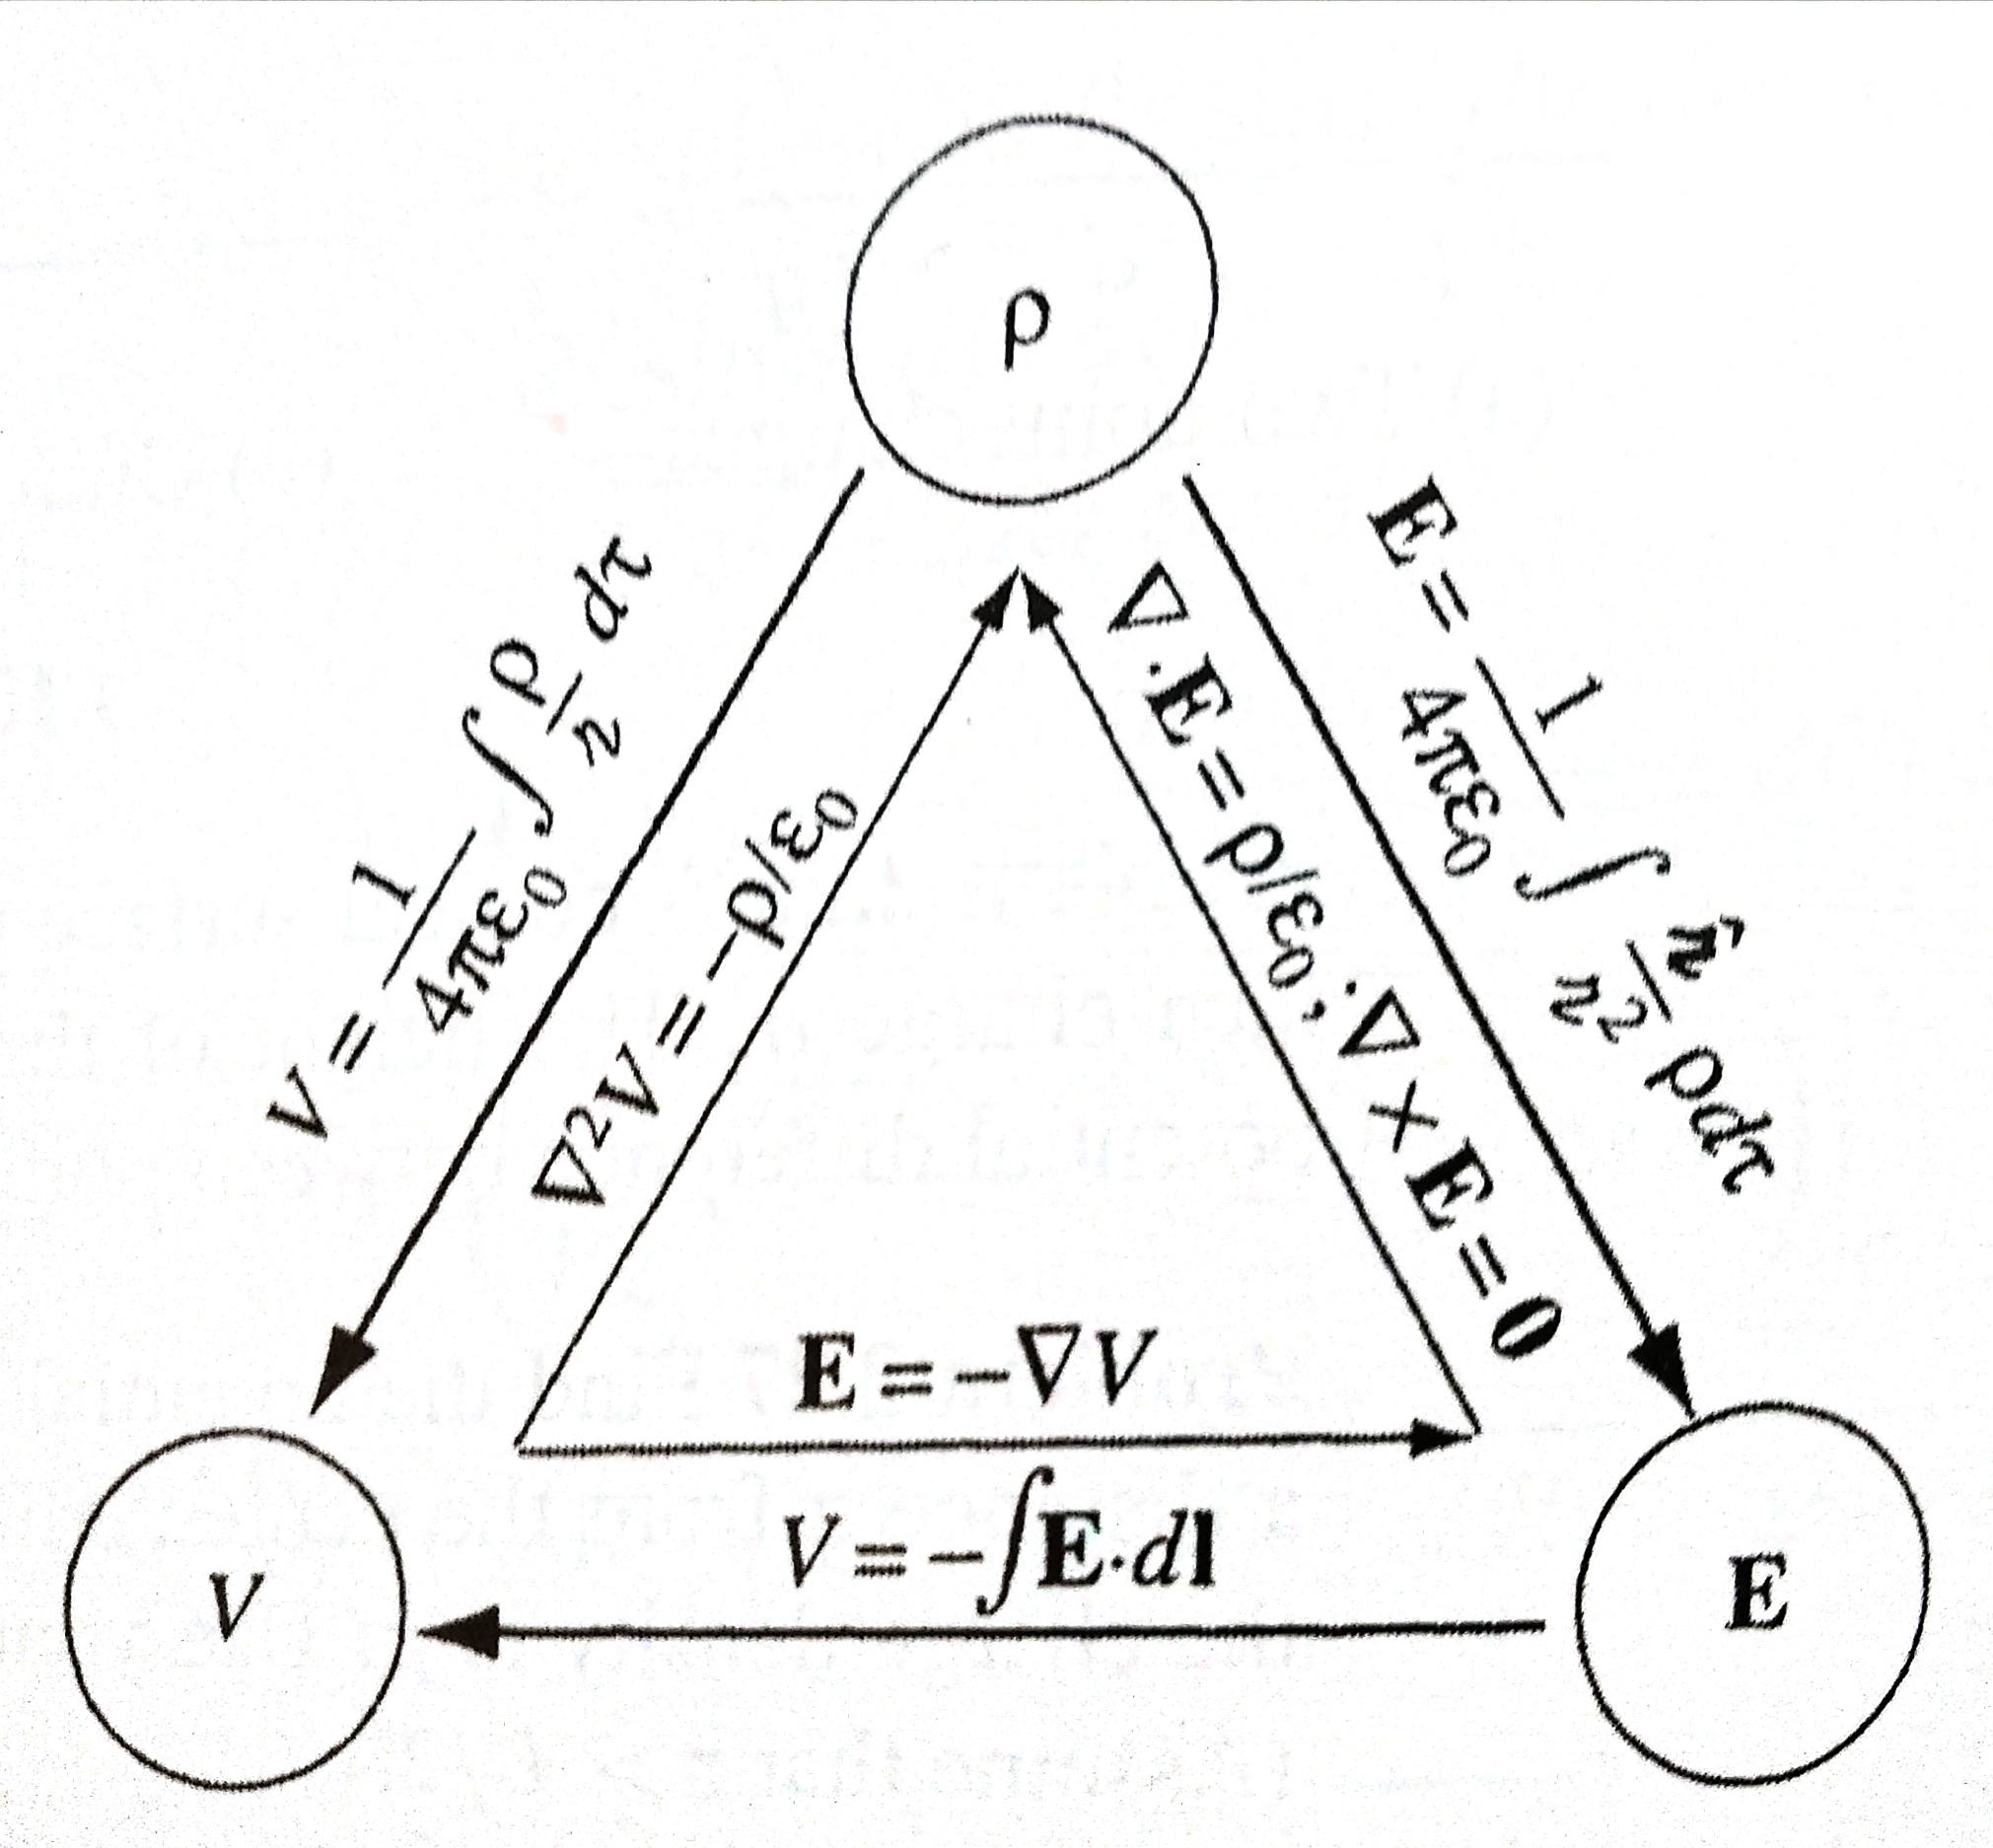
\includegraphics[width=8cm] {img/esummary}
	\end{figure}
	\section{Multipole Expansion of an Electric Potential}
	Let's now develop an approximation for the potential far away from a collection of charge,
	\begin{figure}[H]
		\centering
		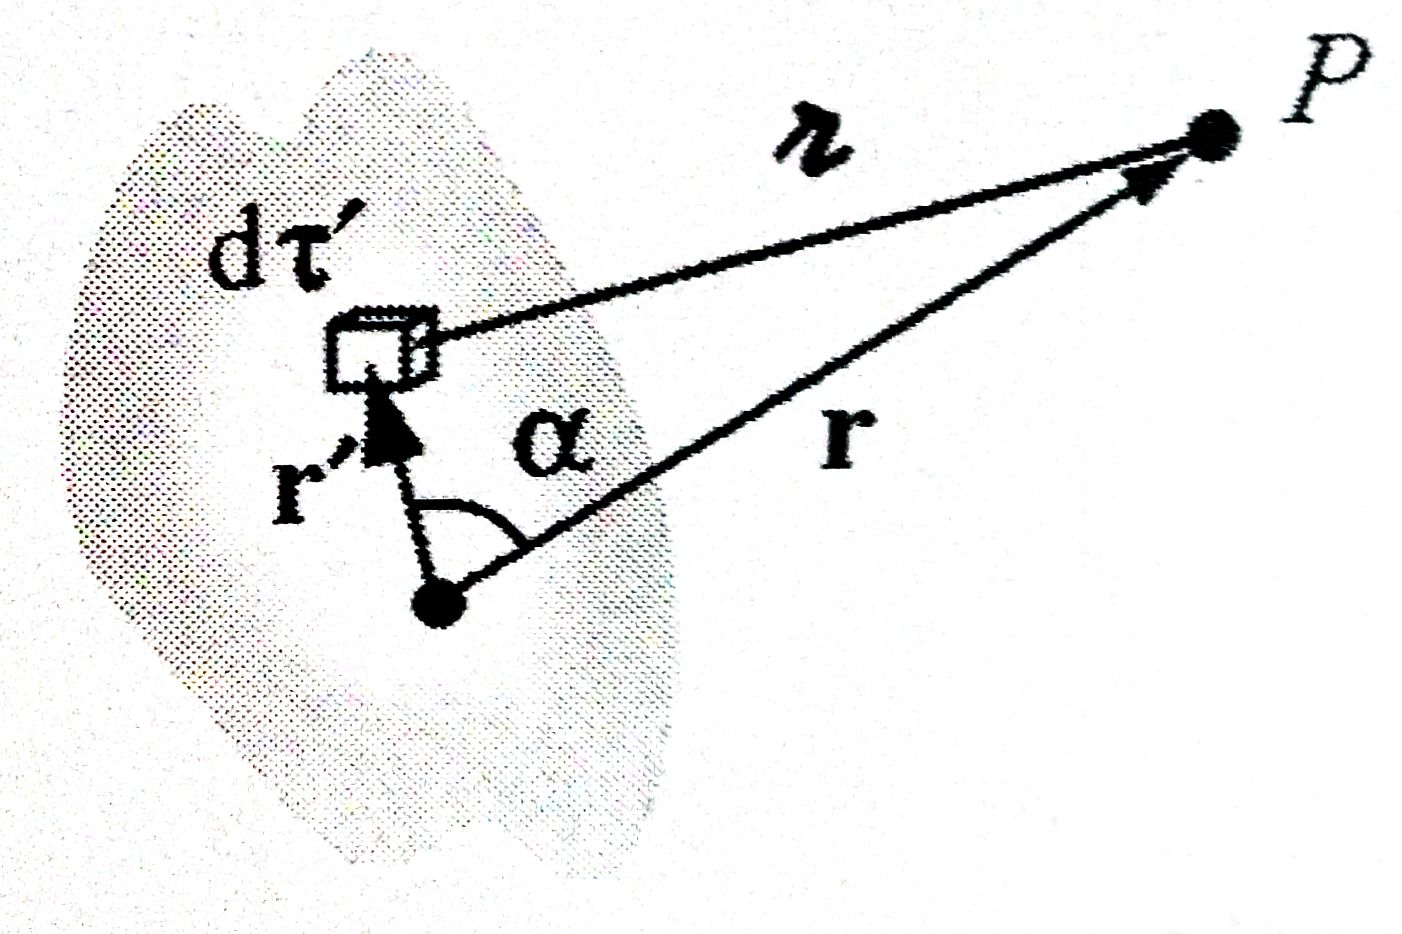
\includegraphics[width=4.5cm] {img/multipole}
	\end{figure}
	Recall that,
	\begin{equation}
		V(\boldsymbol{r}) = \frac{1}{4\pi\epsilon_0} \int_V \frac{\rho(\boldsymbol{r}')}{\rcurs}\ d\tau'
	\end{equation}
	Via the Law of Cosines,
	\begin{equation}
		\rcurs^2 = r^2 + r'^2 - 2rr'\cos\alpha = r^2\left[ 1 + \overbrace{\left(\frac{r'}{r}\right)^2 - 2\left(\frac{r'}{r}\right)\cos\alpha}^\epsilon \right]
	\end{equation}
	\begin{equation}
		\rcurs = r \sqrt{1 + \epsilon};\quad \epsilon = \left(\frac{r'}{r}\right)\left(\frac{r'}{r}- 2\cos\alpha\right)
	\end{equation}
	For large $ r $, $ \epsilon $ is very small. This suggests that we should take the binomial expansion,
	\begin{align}
		\frac{1}{\rcurs} &= \frac{1}{r}\left(1+\epsilon\right)^{-1/2} = \frac{1}{r}\left(1 - \frac{1}{2}\epsilon + \frac{3}{8}\epsilon^2 +\dots \right)\\
		&=\frac{1}{r} \left[ 1 - \frac{1}{2}\left(\frac{r'}{r}\right)\left(\frac{r'}{r}- 2\cos\alpha\right) + \frac{3}{8}\left(\frac{r'}{r}\right)^2\left(\frac{r'}{r}- 2\cos\alpha\right)^2 +\dots \right]\\
		&= \frac{1}{r}\left[1 + \left(\frac{r'}{r}\right)\left(\cos\alpha\right) + \left(\frac{r'}{r}\right)^2\left(\frac{3\cos^2\alpha -1}{2}\right)+\dots\right]\\
		&= \frac{1}{r}\sum_{n=0}^\infty \left(\frac{r'}{r}\right)^n P_n(\cos\alpha) \label{eq:1/rexpand}
	\end{align}
	where $ P_n $ are the Legendre polynomials of order $ n $. Now returning to the potential,
	\begin{equation}
		V(\boldsymbol{r}) = \frac{1}{4\pi\epsilon_0}\int_V \left(\frac{1}{r}\sum_{n=0}^\infty \left(\frac{r'}{r}\right)^n P_n(\cos\alpha)\right)\rho(\boldsymbol{r}')\ d\tau'
	\end{equation}
	\begin{equation}
		\boxed{V(\boldsymbol{r}) = \frac{1}{4\pi\epsilon_0}\sum_{n=0}^\infty \frac{1}{r^{n+1}} \int_V \left(r'\right)^nP_n(\cos\alpha)\rho(\boldsymbol{r})'\ d\tau'}
	\end{equation}
	
	This is the desired multiple expansion. Let's examine the first two terms,
	\begin{equation}
		V(\boldsymbol{r}) = \underbrace{\frac{1}{4\pi\epsilon_0}\frac{1}{r}\int_V \rho(\boldsymbol{r}')\ d\tau' }_\text{monopole}+  \underbrace{\frac{1}{4\pi\epsilon_0}\frac{1}{r^2}\int_Vr'\cos\alpha\  \rho(\boldsymbol{r}')\ d\tau' }_\text{dipole}+ \dots
	\end{equation}
	
	\subsection{Monopole and Dipole Potential}
	We can easily evaluate the integral in the monopole term,
	\begin{equation}
		\boxed{V_\text{mon}(\boldsymbol{r}) = \frac{1}{4\pi\epsilon_0}\frac{Q}{r}}
	\end{equation}
	This makes sense---the first order approximation of the potential at a distance far away is simply that of a point with value of the combined charge.
	
	Now let's examine the dipole term,
	\begin{equation}
		V_\text{dip}(\boldsymbol{r}) = \frac{1}{4\pi\epsilon_0}\frac{1}{r^2}\int_Vr'\cos\alpha\  \rho(\boldsymbol{r}')\ d\tau' 
	\end{equation}
	This form is not very convenient because the $ \alpha $ term contains an $ r $-dependence. In other words, we would have to compute the integral for every field point. Is there any way we can pull the $ r $-dependence outside the integral? If we recognize,
	\begin{equation}
		r'\cos\alpha = \boldsymbol{\hat{r}}\cdot \boldsymbol{r}'
	\end{equation}
	then,
	\begin{equation}
		V_\text{dip}(\boldsymbol{r}) = \frac{1}{4\pi\epsilon_0}\frac{1}{r^2}\boldsymbol{\hat{r}}\cdot \int_V \boldsymbol{r}'\rho(\boldsymbol{r}')\ d\tau'
	\end{equation}
	Now the integral only depends on the field points (i.e. the charge distribution), so we define the dipole moment,
	\begin{equation}
		\boxed{\p= \int_V \boldsymbol{r}'\rho(\boldsymbol{r}')\ d\tau'}
	\end{equation}
	and finally, 
	\begin{equation}
		\boxed{V_\text{dip}(\boldsymbol{r}) = \frac{1}{4\pi\epsilon_0}\frac{\p\cdot \hat{\boldsymbol{r}}}{r^2}}
		\label{eq:dip}
	\end{equation}
	
	The dipole moment for a collection of point charges transforms as expected,
	\begin{equation}
		\p = \sum_{i=1}^n q_i\boldsymbol{r}_i'
	\end{equation}
	
	\subsection{Pure and Physical Dipoles}
	A physical dipole is composed of two equal and opposite point charges ($ \pm q $).
	\begin{figure}[H]
		\centering
		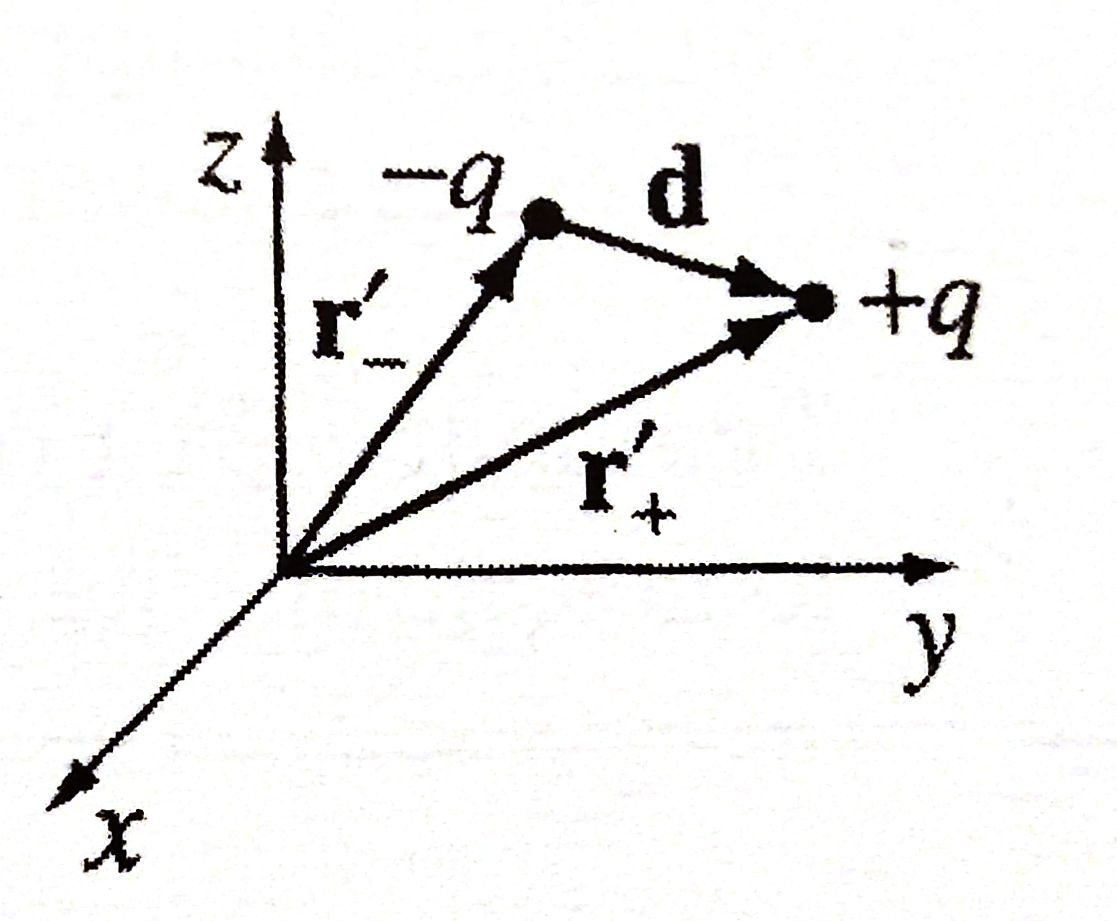
\includegraphics[width=3.5cm] {img/dipole}
	\end{figure}
	We can calculate the dipole moment,
	\begin{equation}
		\p = q\boldsymbol{r}_+' - q\boldsymbol{r}_-' = q\boldsymbol{d}
	\end{equation}
	
	The dipole potential (\ref{eq:dip}) \textit{approximates} the potential of a physical dipole but it is not exact---there are higher order multipole contributions. To construct a pure\footnote{Otherwise known as a perfect or point dipole.} dipole with potential \textit{equal} to \ref{eq:dip}, we must have $ d $ approach zero. In order for the dipole moment to remain nonzero, $ q $ must also tend towards infinity.
	
	\subsection{Origin for Multipole Expansions}
	
	Moving the origin about which we calculate the multipole expansion generally has significant effects on the expansion. For example, a point charge at the origin is a pure monopole but if we were to move the origin then the potential is no longer that of a monopole and will contain higher-order terms. However, note that the monopole moment is the same regardless of the origin because the total charge does not change.
	
	Similarly, a pure dipole has a potential given by \ref{eq:dip} if and only if the dipole is centered on the origin. Unlike the monopole moment ($ Q $), the dipole moment does, in general, change if the origin is moved. An important exception is the case where the total charge is zero. As a quick proof, suppose a charge distribution has dipole moment $ \p_0 $ and we move the origin by an amount $ \boldsymbol{a} $. The new moment, $ \p $, becomes,
	\begin{equation}
		\p = \int_V (\boldsymbol{r}'-\boldsymbol{a})\rho(\boldsymbol{r}')\ d\tau' = \int_V \boldsymbol{r}'\rho(\boldsymbol{r}')\ d\tau' - a\int_V \rho(\boldsymbol{r}') = \p_0 - Q\boldsymbol{a}
	\end{equation}
	Thus, $ \p=\p_0 $ if $ Q=0 $.
	
	\section{Electric Fields in Matter}
	Dielectric materials contain microscopic ``natural" dipoles (i.e. polar molecules) and dipoles induced by an external electric field. We can quantify the local polarization of charge with the quantity of polarization, $ \P $\footnote{This convention of $ \p $ and $ \P $ is not ideal\dots}, which is defined to be the dipole moment per unit volume.
	
	\subsection{Bound Charge}
	Suppose we have  a material with polarization. Our first task is to calculate the field produced by the polarization\footnote{Note: not the field the causes the polarization but the field that results from the polarization.},
	\begin{equation}
		V(\boldsymbol{r}) = \frac{1}{4\pi\epsilon_0}\int_V \frac{\P(\boldsymbol{r}')\cdot \hat{\brcurs}}{\rcurs^2}\ d\tau'
	\end{equation}
	where $ \brcurs $ is the vector from the local dipole to the field point.
	
	While this expression is valid, in the following section, we shall embark on a series of rather not-intuitive steps to cast $ V(\boldsymbol{r}) $ in a more interesting light. To begin, recall (Appendix \ref{appendix:aside2}),
	\begin{equation}
		\grad'\left(\frac{1}{\rcurs}\right) = \frac{\hrcurs}{\rcurs^2}
		\label{eq:div1/r}
	\end{equation}
	Thus,
	\begin{equation}
		V(\boldsymbol{r}) = \frac{1}{4\pi\epsilon_0}\int_V \P(\boldsymbol{r}')\cdot\grad'\left(\frac{1}{\rcurs}\right)\ d\tau'
	\end{equation}
	Integrating by parts,
	\begin{equation}
		V(\b{r}) = \frac{1}{4\pi\epsilon_0}\left[\int_V \grad'\cdot\left(\frac{\P}{\rcurs}\right)\ d\tau' - \int_V \frac{1}{\rcurs}\left(\grad' \cdot\P\right) \ d\tau'\right]
	\end{equation}
	Invoking the Divergence Theorem\footnote{Up until now, I have followed Griffiths closely. Here I will adapt Jackson's approach: he takes the volume of integration to be all of space so that the first term drops out. In contrast, Griffiths takes the volume to be the dielectric. In Jackson's case, it is easier to justify that the total bound charge has value $ -\div\P $ while in Griffiths' case, the bound charge is delineated into bound charge within the dielectric ($ \rho_b = -\div\P $) and surface charge at the surface of the dielectric ($ \sigma_b = \P\cdot\unit{n} $).},
	\begin{equation}
		V = \frac{1}{4\pi\epsilon_0}\oint_S \cancel{\frac{\left(\P\cdot\unit{n}\right)}{\rcurs}}\ da' + \frac{1}{4\pi\epsilon_0} \int_V \frac{\left(-\grad'\cdot\P\right)}{\rcurs}\ d\tau'
	\end{equation}
	We see that the remaining term in parenthesis behaves as a volume charge. This is the bound charge that results from non-uniform polarization.
	\begin{equation}
		\boxed{\rho_b = -\div\P}
	\end{equation}
	Thus,
	\begin{equation}
		\boxed{		V(\b{r}) = \frac{1}{4\pi\epsilon_0}\int_V \frac{\rho_b}{\rcurs}\ d\tau'}
	\end{equation}
	
	The potential produced by the polarized material is the same as that produced by the bound\footnote{Bound because the charge can not be removed from the atom or molecule onto which it is attached.} charges. Note that these charges are not fictitious (i.e. just for bookkeeping), but rather, real accumulations of charge\footnote{Griffiths Section 4.2.2 has a great interpretation.}.
	
	\subsection{Electric Displacement}
	Within a dielectric, the total charge density can be written as,
	\begin{equation}
		\rho = \rho_f +\rho_b
	\end{equation}
	where $ \rho_f$ is the free charge: charge that is not a result of polarization. Now, let's return to Gauss's Law,
	\begin{equation}
		\div \E = \frac{\rho}{\epsilon_0} =  \frac{ \rho_f +\rho_b}{\epsilon_0}  = \frac{\rho_f -\div\P}{\epsilon_0} 
	\end{equation}
	\begin{equation}
		\div \left(\epsilon_0\E + \P\right) = \rho_f
	\end{equation}
	Let's define the electric displacement,
	\begin{equation}
		\boxed{\b{D} = \epsilon_0\E + \P}
	\end{equation}
	where,
	\begin{equation}
		\boxed{\div\b{D}= \rho_f}
	\end{equation}
	While the displacement field seems to parallel the total electric field, there is one important distinction: the displacement is not irrotational,
	\begin{equation}
		\curl \b{D} = \curl \left(\epsilon_0\E + \P\right) = \epsilon_0\cancel{\curl \E } \ + \curl \P
	\end{equation}
	\begin{equation}
		\boxed{\curl \b{D} = \curl \P}
	\end{equation}
	In other words, while the total electric field $ \E $ is generated only by total charge $ \rho $, the electric displacement field $ \b{D} $ is not entirely generated by free charge $ \rho_f $.
	
	\subsection{Linear Dielectrics}
	In materials that are linear dielectrics, it is often sufficient to approximate the polarization as proportional to the total field,
	\begin{equation}
		\P = \epsilon_0\chi_e \E
	\end{equation}
	Where the dimensionless constant of proportionality, $ \chi_e $ is the electric susceptibility. Note that $ \E $ is the total field. If we were to place a linear dielectric in some external field $ \E' $, we \textit{can not }use the equation above to calculate the polarization: the external field will polarize the material, which will change the total field, which will change the polarization, which will change the total field\ldots
	
	One way to break out of this infinite loop is to calculate $ \b{D} $ from the free charge (this is generally quite challenging but nevertheless viable in certain situations). In this case, let's calculate the displacement field,
	\begin{equation}
		\b{D} = \epsilon_0\E + \P = \epsilon_0\E + \epsilon_0\chi_e\E
	\end{equation}
	\begin{equation}
		\boxed{\b{D} = \epsilon\E;\quad \epsilon\equiv \epsilon_0 \left(1 + \chi_e\right)}
	\end{equation}
	where $ \epsilon_0 $ is the permittivity of free space and $ \epsilon $ is the permittivity of a linear dielectric. We can also define the dielectric constant, otherwise known as the relative permittivity,
	\begin{equation}
		\epsilon_r \equiv \epsilon/\epsilon_0 = 1+\chi_e
	\end{equation}
	
	\chapter{Magnetostatics}
	
	While stationary charges only produce and electric field, moving charges generate an additional magnetic field. In this section we will examine magnetostatics: time-constant magnetic fields produced by steady currents. This is the next big area of study in electrodynamics\footnote{More like electro-not-dynamics at this point.} having already covered it's counterpart, electrostatics: time-constant electric fields generated by stationary charges.
	
	Before moving forwards, let's clarify what we mean by a steady current. To begin, a current, $ \b{I}$, in an infinitely-thin wire has a magnitude equal to the charge per unit time passing a given point in the wire. In two dimensions, the surface current density, $ \b{K} $, has magnitude equal to the current per unit width; and in three dimensions, the volume current density, $ \b{J} $, has magnitude equal to the current per unit area\footnote{A misconception I had for some time: $ (\b{J}\ d\tau)\neq d\b{I} $ nor $ (\b{J} \ d\tau)\neq dQ $}.
	
	We can derivative a continuity relation for $ \b{J} $. For some closed surface $ S $, the current crossing the surface, 
	\begin{equation}
		I = \oint_S \b{J}\cdot d\b{a} = \int_V \left(\div \b{J}\right)\ d\tau
	\end{equation}
	In addition, because charge is conserved, current flowing out implies that charge inside the surface is decreasing,
	\begin{equation}
		I = -\dv{}{t}\int_V \rho\ d\tau = -\int_V \left(\pdv{\rho}{t}\right)\ d\tau
	\end{equation}
	Thus, combining the two results above,
	\begin{equation}
		\boxed{\div \b{J} =-\pdv{\rho}{t} }
	\end{equation}
	
	Returning to \textit{steady} currents: a constant flow of charge for all space and time without charge piling up anywhere. This corresponds to the conditions that\footnote{Notice the last terms results from applying results from the second term to the continuity equation.},
	\begin{equation}
		\pdv{\b{J}}{t}=0;\quad \pdv{\rho}{t} = 0; \quad \div \b{J} = 0
	\end{equation}
	
	In practice, currents are never steady, just as charges are never truly stationary for all time. However, at any instant in time, it is often a sufficient approximation to treat currents and charges as stationary.
	
	\section{Magnetostatic Field}
	
	The Biot-Savart Law gives the magnetic field generated by a steady line current oriented along a curve $ C $,
	\begin{equation}
		\B(\b{r}) = \frac{\mu_0}{4\pi}\int_C \frac{\b{I}(\b{r'})\cross \hrcurs}{\rcurs^2}\ dl'
	\end{equation}
	
	Notice that, our current is for a wire without thickness. We can generalize the equation above by expressing current in terms of $ \b{J} $,
	\begin{equation}
		\boxed{\B(\b{r}) = \frac{\mu_0}{4\pi}\int_V \frac{\b{J}\b{(r')}\cross \hrcurs}{\rcurs^2}\ d\tau'}
	\end{equation}
	
	The magnetic force on a charge $ q $ with velocity $ \b{v} $ in a magnetic field $ \B $ is given by the Lorentz Law,
	\begin{equation}
		\boxed{\b{F} = q(\b{v}\cross \B)}
	\end{equation}
	
	\subsection{Divergence of a Magnetostatic Field}
	
	We can calculate the divergence of the magnetic field given by the Biot-Savart Law,
	\begin{align}
		\div \B &= \div \left( \frac{\mu_0}{4\pi}\int_V \frac{\b{J}\b{(r')}\cross \hrcurs}{\rcurs^2}\ d\tau'\right)\\
		&= \frac{\mu_0}{4\pi}\int_V  \div \left(\b{J}\b{(r')}\cross \frac{\hrcurs}{\rcurs^2}\right)\ d\tau'\\
		&= \frac{\mu_0}{4\pi} \left[ \frac{\hrcurs}{\rcurs^2}\cdot \left(\cancel{\curl \b{J}(\b{r'})}\right) - \b{J}(\b{r'})\cdot \left(\cancel{\curl \frac{\hrcurs}{\rcurs^2}}\right)  \right] = 0
	\end{align}
	The first term is zero because $ \b{J}(\b{r}') $ does no depend on $ \b{r} $ and the second term is zero by calculation (or inspection).
	\begin{equation}
		\boxed{\div \B = 0}
	\end{equation}
	
	\subsection{Curl of a Magnetostatic Field}
	Similarly, we can calculate the curl of the magnetic field,
	\begin{align}
		\curl \B &= \curl \left( \frac{\mu_0}{4\pi}\int_V \frac{\b{J}\b{(r')}\cross \hrcurs}{\rcurs^2}\ d\tau'\right)\\
		&= \frac{\mu_0}{4\pi}\int_V  \curl \left(\b{J}\b{(r')}\cross \frac{\hrcurs}{\rcurs^2}\right)\ d\tau'\\
		&= \frac{\mu_0}{4\pi}\int_V \left[ \cancel{\left(\frac{\hrcurs}{\rcurs^2}\cdot\nabla\right)\b{J}} - \left(\b{J}\cdot\nabla\right) \frac{\hrcurs}{\rcurs^2} + \b{J} \left(\div \frac{\hrcurs}{\rcurs^2}\right) - \frac{\hrcurs}{\rcurs^2}\cancel{\left(\div \b{J} \right)}\right]\ d\tau' \label{eq:curl1} \\
		&= -\frac{\mu_0}{4\pi}\int_V \left(\b{J}\cdot\nabla\right) \frac{\hrcurs}{\rcurs^2}\ d\tau' + \frac{\mu_0}{4\pi}\int_V \b{J}(\b{r}') \left(4\pi\delta(\brcurs)\right)\ d\tau' \\
		&= -\frac{\mu_0}{4\pi}\int_V \left(\b{J}\cdot\nabla\right) \frac{\hrcurs}{\rcurs^2}\ d\tau' + \mu_0\b{J}(\b{r})
	\end{align}
	For the sake of brevity, I will simply state that the first term in the expression above will evaluate to zero \textit{assuming steady currents} ($ \div\b{J} =0 $). Thus,
	\begin{equation}
		\boxed{\curl \B = \mu_0 \b{J}}
	\end{equation}
	We can derive Amp\`ere's Law by applying Stokes' Theorem for a closed loop, 
	\begin{equation}
		 \oint_C \B\cdot d\b{l} = \int_S \left(\curl\B\right)\cdot d\b{a} =\int_S  \mu_0\b{J} \cdot d\b{a}
	\end{equation}
	\begin{equation}
		\boxed{\oint_C \B\cdot d\b{l} = \mu_0 I_\text{enc}}
	\end{equation}
	where $ I_\text{enc} $ is the current passing through the Amperian loop. Like Gauss's Law,  Amp\`ere's Law is generally only useful in systems with high degrees of symmetry.
	
	\section{Magnetic Vector Potential}
	Just as $ \curl \E =0$ prompted the formulation of the electric potential, $ \div \B =0$ suggests we should introduce a magnetic vector potential $ \b{A} $ such that,
	\begin{equation}
		\B = \curl \b{A}
	\end{equation}
	Now, just as we can express the electric potential as a function of charge, we wish to express magnetic potential as a function of current. Let's first develop some relations that will help us in this endeavor. From Appendix \ref{appendix:aside2},
	\begin{equation}
		\grad\left(\frac{1}{\rcurs}\right) =-\frac{\hrcurs}{\rcurs^2}
	\end{equation}
	Furthermore,
	\begin{equation}
		\curl(\frac{1}{\rcurs}\b{J}) = \left[\grad \left(\frac{1}{\rcurs}\right)\cross\b{J} \right]+ \left[\frac{1}{\rcurs}\left(\curl\b{J}\right)\right]
	\end{equation}
	Thus, combining everything with our expression for $ \b{B} $,
	\begin{align}
		\B &= \frac{\mu_0}{4\pi}\int_V \frac{\b{J}\cross \hrcurs}{\rcurs^2}\ d\tau'\\
		&= \frac{-\mu_0}{4\pi}\int_V \b{J}\cross \grad\left(\frac{1}{\rcurs}\right)\ d\tau'\\
		&= \frac{\mu_0}{4\pi}\int_V \left( \curl(\frac{1}{\rcurs}\b{J}(\b{r}')) -  \frac{1}{\rcurs}\left(\cancel{\curl\b{J}}\right)\right)\ d\tau'\\
		&= \curl \left(\frac{\mu_0}{4\pi}\int_V  \frac{\b{J}(\b{r}')}{\rcurs}\ d\tau'\right)
	\end{align}
	Thus,
	\begin{equation}
		\boxed{\b{A} = \frac{\mu_0}{4\pi}\int_V  \frac{\b{J}(\b{r}')}{\rcurs}\ d\tau'}
		\label{eq:p3}
	\end{equation}
	\subsection{Gauge Transformations}
	Recall that, in the previous section, we noticed the the electric potential is unique up to a constant scalar field. Similarly, the vector potential is unique up to vector field with no curl. In other words---keeping in mind the fact that the curl of a gradient is always zero---we can define a \textit{gauge} $ \grad \psi $ such that the magnetic field is invariant under the transformation,
	\begin{equation}
		\b{A} \to \b{A} - \grad\psi
	\end{equation}
	This property is known as \textit{gauge invariance} and suggests that we free to choose the most convenient gauge to a potential. For the vector potential, we would like for the divergence of $ \b{A} $ to be zero, but is there guaranteed to be a gauge such that $ \div\b{A} =0$? Suppose we find some vector potential $ \b{A}_0 $ that has a divergence. Next, let's define $ \b{A} =  \b{A}_0 + \grad\psi$,
	\begin{align}
		\div\b{A}  &= \div \left(\b{A}_0  + \grad\psi\right)\\
		&= \div \b{A}_0  + \laplacian{\psi}
	\end{align}
	If $ \div\b{A} =0 $, then
	\begin{equation}
		 \laplacian{\psi} = \div \b{A}_0
	\end{equation}
	This is Poisson's equation, which we know has an unique solution (given appropriate boundary conditions)! Thus, there does in fact exists a gauge where the $ \div \b{A} =0 $. This is known as the \textit{Coulomb gauge},
	\begin{equation}
		\boxed{\curl\b{A} = \B;\qquad\div\b{A}=0}
	\end{equation}

	In the Coulomb gauge, we notice that,
	\begin{equation}
		\curl\B = \curl \left(\curl\b{A}\right) = \grad \left(\cancel{\div \b{A}}\right) - \laplacian{\b{A}} = \mu_0\b{J}
	\end{equation}
	\begin{equation}
		\boxed{\laplacian{\b{A}} = -\mu_0\b{J}}
		\label{eq:p4}
	\end{equation}
	
	Notice the parallels between eq. \ref{eq:p1} and \ref{eq:p2} with eq. \ref{eq:p3} and \ref{eq:p4}.
	
	\subsection{Summary of Magnetostatic Relations}
	\begin{figure}[H]
		\centering
		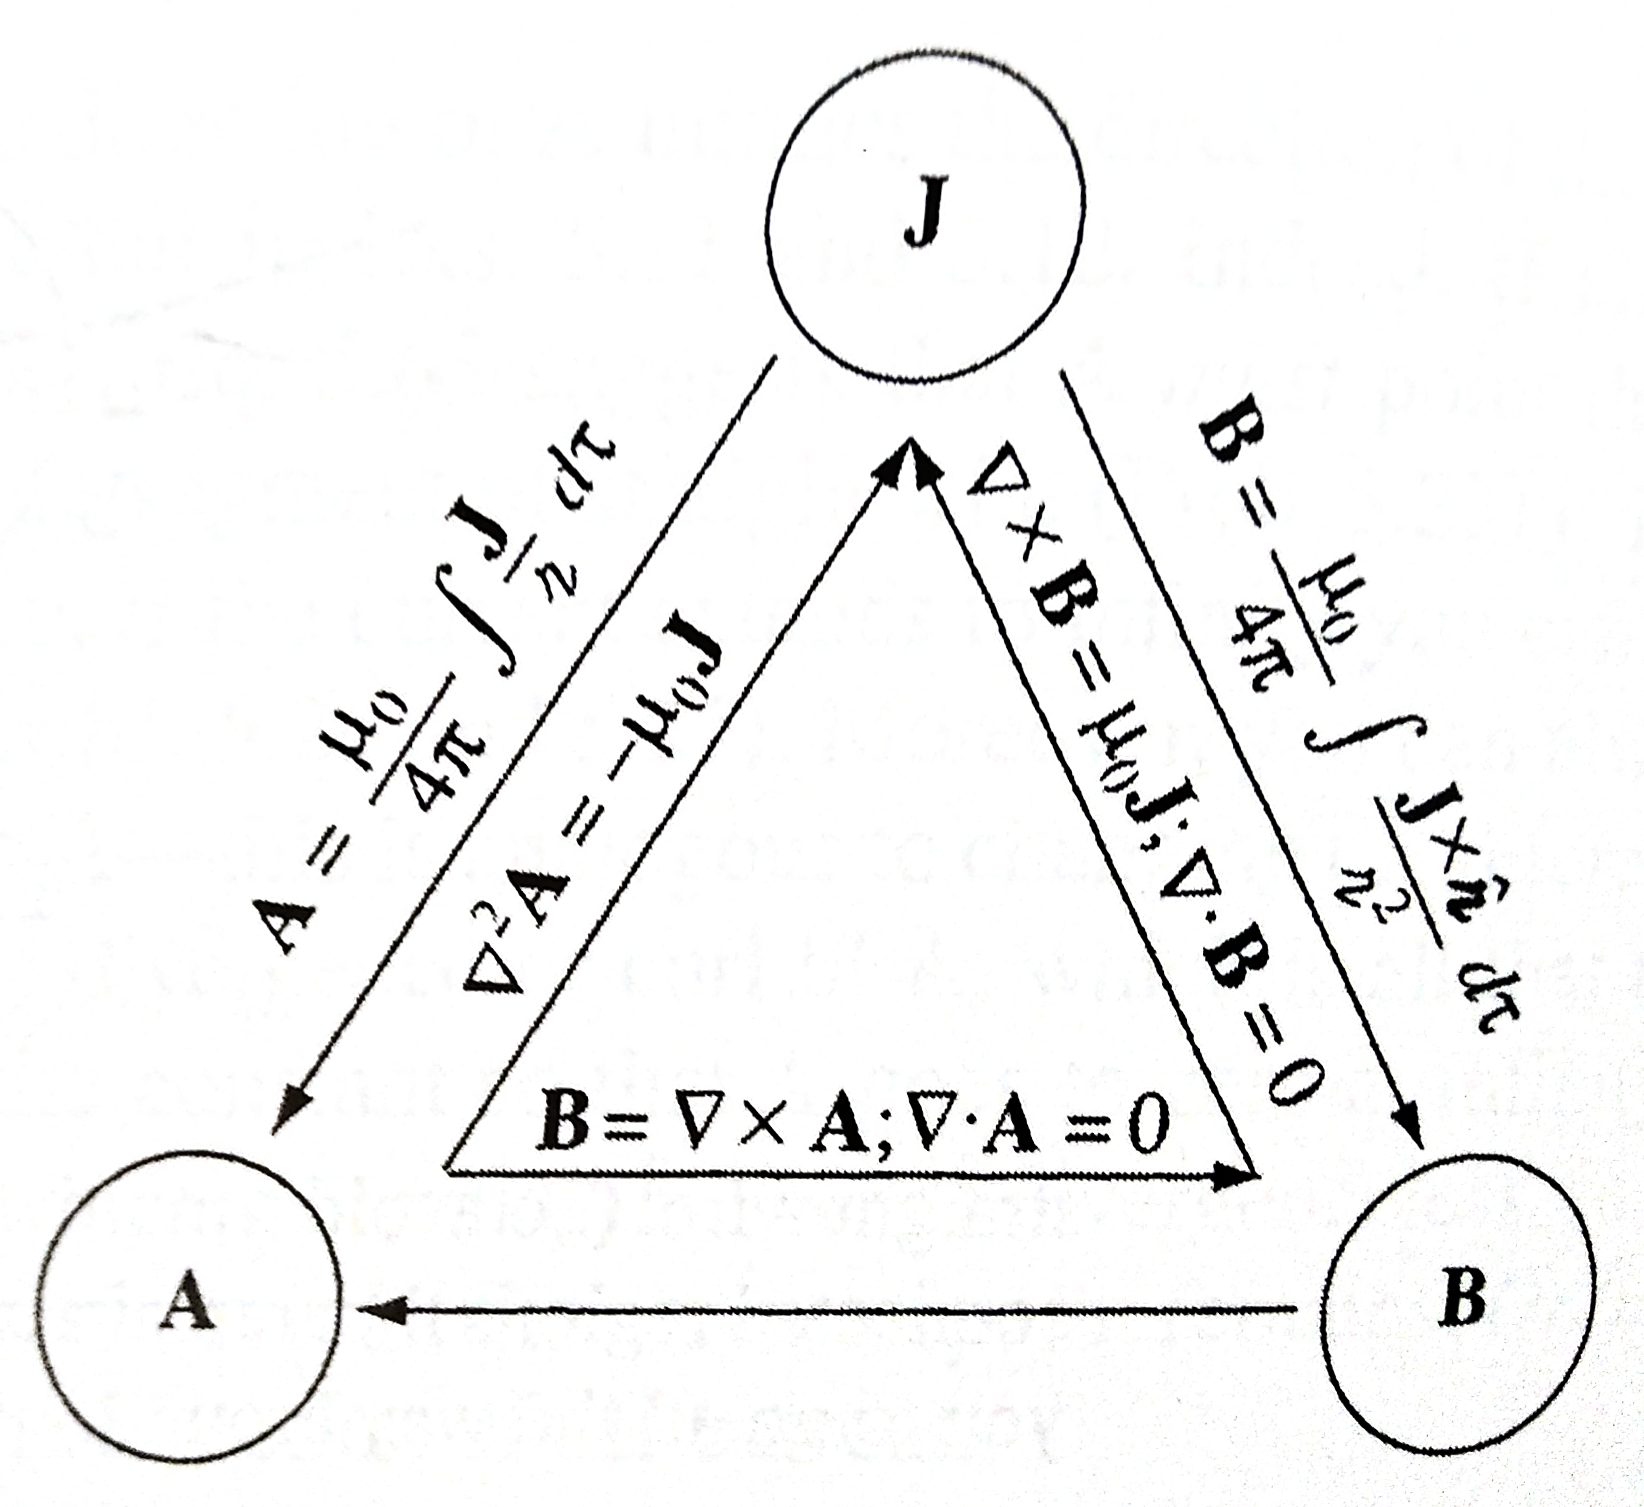
\includegraphics[width=8cm] {img/bsummary}
	\end{figure}
	
	\section{Multipole Expansion of a Magnetic Vector Potential}
	\begin{figure}[H]
		\centering
		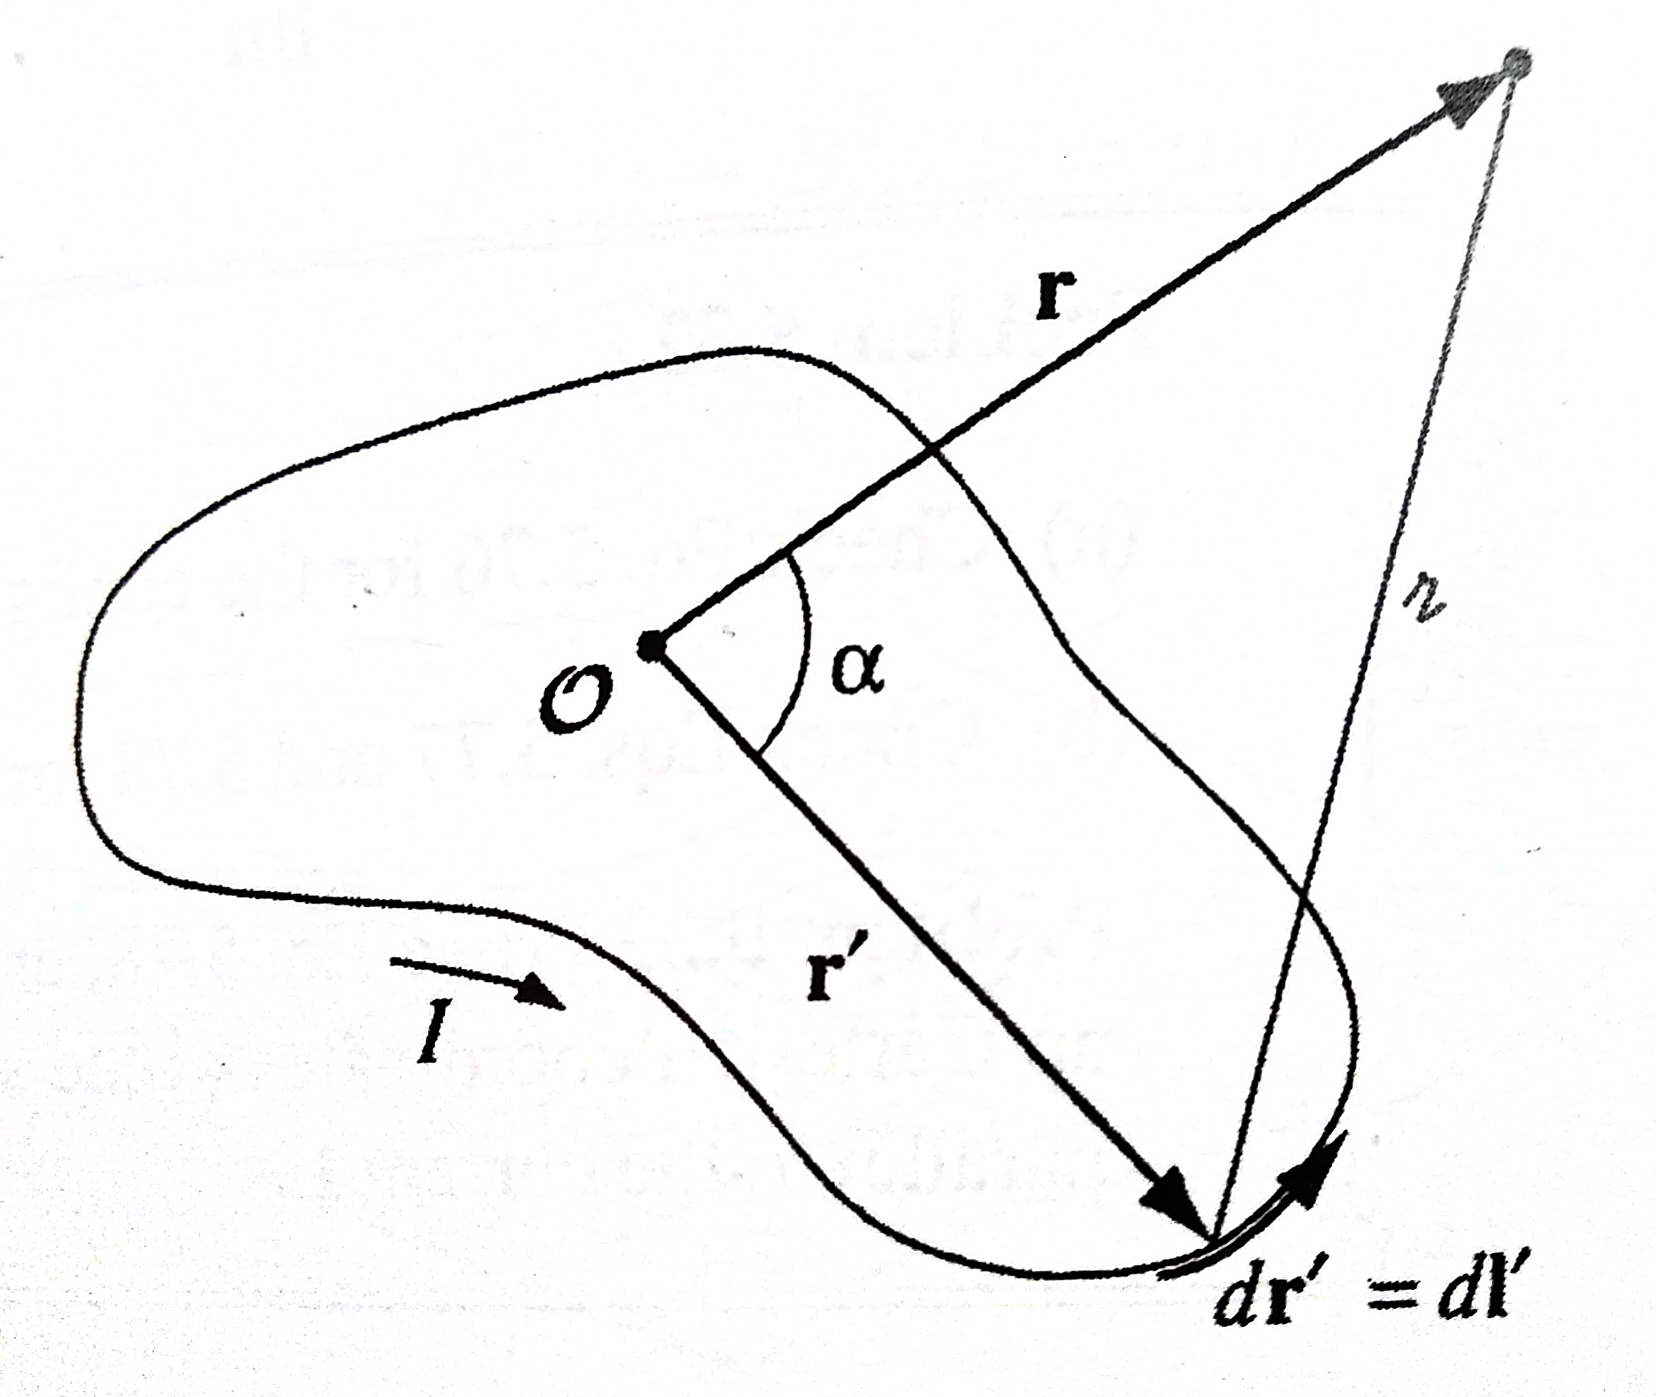
\includegraphics[width=5cm] {img/magmultipole}
	\end{figure}
	We now wish to derive an approximate formula for the vector potential of a localized current distribution that is valid a large distance away. Recall that in the electric multipole expansion, we found (eq. \ref{eq:1/rexpand}),
	\begin{equation}
		\frac{1}{\rcurs} = \frac{1}{r}\sum_{n=0}^\infty \left(\frac{r'}{r}\right)^n P_n(\cos\alpha) 
	\end{equation}
	Recall,
	\begin{equation}
		\b{A}(\b{r}) = \frac{\mu_0}{4\pi}\oint_C \frac{\b{I}}{\rcurs}\ dl'
	\end{equation}	
	Thus (recall the current is steady, so we can pull $ I $ out of the equation),
	\begin{equation}
		\boxed{\b{A}(\b{r}) = \frac{\mu_0 I}{4\pi}\sum_{n=0}^\infty \frac{1}{r^{n+1}} \oint_C (r')^n P_n(\cos\alpha)\ d\b{l}'}
	\end{equation}
	
	\subsection{Monopole and Dipole Potential}
	Let's now examine the first two terms of the multipole expansion,
	\begin{equation}
		\b{A}(\b{r}) = \underbrace{\frac{\mu_0 I}{4\pi}\frac{1}{r}\oint_C d\b{l}'}_\text{monopole} + \underbrace{ \frac{\mu_0 I}{4\pi}\frac{1}{r^2}\oint_C r'\cos\alpha \ d\b{l}'}_\text{dipole}
	\end{equation}
	The monopole term is always zero because the vector displacement around a closed loop,
	\begin{equation}
		\oint_C d\b{l}' = 0
	\end{equation}
	Thus,
	\begin{equation}
		\boxed{\b{A}_\text{mon}(\b{r}) = 0}
	\end{equation}
	
	This, once again, reflects the idea that there does not exists magnetic monopoles.
	
	Now, let's turn to the dipole term\footnote{The justification for the final manipulation can be found in Griffiths' problems 1.61 and 1.62.},
	\begin{align}
		\b{A}_\text{dip}(\b{r}) &=  \frac{\mu_0 I}{4\pi}\frac{1}{r^2}\oint_C r'\cos\alpha \ d\b{l}'\\
		&=  \frac{\mu_0 I}{4\pi}\frac{1}{r^2}\oint_C \left(\hrcurs\cdot\b{r}'\right)\ d\b{l}'\\
		&= \frac{\mu_0 I}{4\pi}\frac{1}{r^2} \left(-\hrcurs\cross\int_S d\b{a}'\right)
	\end{align}
	We can separate this equation into a source component and a field component,
	\begin{equation}
		\boxed{\b{A}_\text{dip}(\b{r}) =  \frac{\mu_0}{4\pi}\frac{\b{m}\cross\hrcurs}{r^2}}
		\label{eq:adip}
	\end{equation}
	where $ \b{m} $ is the magnetic dipole moment,
	\begin{equation}
		\boxed{\b{m} = I\int_S d\b{a}'}
	\end{equation}
	Note that the integral terms is the \textit{vector area}. For a flat loop, the vector area is the ordinary area enclosed with direction given by the right-hand rule. Also note that the dipole moment is independent of origin. This is not the case for the electric dipole moment.
	
	\subsection{Pure and Physical Dipole}
	A physical magnetic dipole, a loop of current, generally contains higher potential terms. Like the electric analog, we can devise a pure magnetic dipole with potential exactly equal to the dipole potential by taking an infinitesimally small loop at the origin with with the current tending towards infinity so that the dipole moment does not cancel. 
	
	\section{Magnetic Fields in Matter}
	
	Returning to atomic model of matter, we simply state that the spin and orbital motion of electrons in matter generates magnetic dipole moments that tend to align both parallel (paramagnetic) and opposite (diamagnetic) relative to the total magnetic field $ \B $. We define the \textit{magnetization}, $ \M $, as the magnetic dipole moment per unit volume.
	
	\subsection{Bound Currents}
	What is the magnetic field produced by an object with known magnetization, $ \M $? From eq. \ref{eq:adip},
	\begin{equation}
		\b{A}(\b{r}) = \frac{\mu_0}{4\pi} \int_V \frac{\M(\b{r}')\cross\hrcurs}{\rcurs^2}\ d \tau'
	\end{equation}
	As in the electric case (eq. \ref{eq:div1/r}),
	\begin{equation}
		\grad'\left(\frac{1}{\rcurs}\right) = \frac{\hrcurs}{\rcurs^2}
	\end{equation}
	so,
	\begin{align}
			\b{A}(\b{r}) &= \frac{\mu_0}{4\pi}\int_V \left(\M(\b{r}')\ \cross \grad'\left(\frac{1}{\rcurs}\right) \right)\ d\tau'\\
			&= \frac{\mu_0}{4\pi} \int_V \frac{1}{\rcurs}\left[\grad'\cross \M(\b{r}')\right]\ d\tau' - \frac{\mu_0}{4\pi}\int_V\grad '\cross \left(\frac{\M(\b{r}')}{\rcurs}\right)\ d \tau'\\
			&=  \frac{\mu_0}{4\pi} \int_V \frac{1}{\rcurs}\left[\grad'\cross \M(\b{r}')\right]\ d\tau' - \frac{\mu_0}{4\pi}\cancel{\oint_S \frac{1}{\rcurs} \left[\M(\b{r}')\cross d \b{a}'\right]}
	\end{align}
	Notice that we manipulated the equations above using the product role and other vector identities developed in Griffiths\footnote{Griffiths problem 1.61.}. As in the electric case, we follow Jackson rather than Griffiths in choosing our volume of integration to be all space so that the surface integral cancels. Notice the the remaining term resembles a current density. Thus, we define the bound current,
	\begin{equation}
		\boxed{\b{J}_\text{b} = \curl{\M}}
	\end{equation}
	such that the vector potential produced by the magnetization (not the total potential) becomes,
	\begin{equation}
		\boxed{\b{A}(\b{r}) = \frac{\mu_0}{4\pi} \int_V  \frac{\b{J}_\text{b}(\b{r}')}{\rcurs}\ d\tau'}
	\end{equation}
	
	\subsection{Auxiliary Field}
	We can separate the total current into to parts: the bound current we just discussed and the remaining---free---current.
	\begin{equation}
		\boxed{\b{J} = \bd{J}_\text{b} + \bd{J}_\text{f}} 
	\end{equation}
	Amp\`ere's law can be written as,
	\begin{equation}
		(1/\mu_0)\curl \B = \bd{J} = \bd{J}_\text{b} + \bd{J}_\text{f} = \left(\curl\M\right)+ \bd{J}_\text{f} 
	\end{equation}
	\begin{equation}
		\curl \left(\frac{1}{\mu_0}\B - \M\right) =  \bd{J}_\text{f} 
	\end{equation}
	Thus, we can define the Auxiliary Field $ \H $, 
	\begin{equation}
		\boxed{\H = \frac{1}{\mu_0}\B - \M}
	\end{equation}
	where,
	\begin{equation}
		\boxed{\curl \H = \bd{J}_\text{f}}
	\end{equation}
	While $ \H $ resembles $ \B $ for free currents, and important difference between the magnetic and auxiliary is presented below,
	\begin{equation}
		\div \H  = \div \left(\frac{1}{\mu_0}\B - \M\right) = \frac{1}{\mu_0}\cancel{\div \B }- \div \M
	\end{equation} 
	\begin{equation}
		\boxed{\div\H = -\div \M}
	\end{equation}
	Unlike that magnetic field, the divergence of the auxiliary field is, in general, nonzero. As a corollary, we can not assume $ \H=0 $ just because there is no free current.
	
	\subsection{Linear and Nonlinear Media}
	In paramagnetic and diamagnetic materials, it is often a good approximation that the magnetization is proportion to the magnetic field,
	\begin{equation}
		\boxed{\M = \chi_m\H}
	\end{equation}
	Where the dimensionless quantity $ \chi_m $ is the magnetic susceptibility that is position for paramagnets and negative for diamagnets. For such \textit{linear media},
	\begin{equation}
		\B = \mu_o (\H + \M) = \mu_0 (\H + \chi_m\H)
	\end{equation}
	thus,
	\begin{equation}
		\boxed{\B = \mu\H;\quad \mu = \mu_0(1+\chi_m)\H}
	\end{equation}
	where $ \mu_0 $ is the permeability of free space and $ \mu $ is the permeability of the material.
	
	Ferromagnetism is another interesting topic, but beyond the scope of this document.
	
	\section{Maxwell's Equations for Electrostatics}
	Combining our results from the previous two sections,
	\begin{empheq}[box=\fbox]{align}
		\begin{aligned}
		&\div \E = \frac{1}{\epsilon_0}\rho\qquad&
		&\div \B= 0
		\\
		&\curl \E = 0\qquad&
		&\curl \B = \mu_0\b{J}
		\end{aligned}
	\end{empheq}
	These equations must be supplement by appropriate boundary conditions in order to find a unique solution. Following the Helmholtz Theorem, it is generally implicit that we assume the conditions $ \E,\B\to 0 $ far away from all charges and currents.
	
	Physically, we can interpret these equations as: electric fields originate at positive charges and terminate at negative charges while magnetic fields can not begin nor end anywhere. In other words, there are no ``magnetic charges" (magnetic monopoles).
	
	\newpage
	\begin{table}[ht!]
		\centering
		\def\arraystretch{2.5}
		\caption{Summary of Electro-Magneto Statics}
		\vspace{1em}
		\begin{tabular}{l| c| c }
			\hline
			\textbf{Property} & \textbf{Electrostatic} & \textbf{Magnetostatic} \\
			\hline\hline
			Force & $\b{F} = q\E$ & $\b{F} = q\left(\b{v}\cross \B\right)$\\
			\hline
			Field &  $\displaystyle\boldsymbol{E}(\boldsymbol{r}) = \frac{1}{4\pi\epsilon_0}\int_V \frac{\rho(\boldsymbol{r}')}{\rcurs^2}\hat{\brcurs}\,d\tau'$& $\displaystyle\B(\b{r}) = \frac{\mu_0}{4\pi}\int_V \frac{\b{J}\b{(r')}\cross \hrcurs}{\rcurs^2}\ d\tau'$\\[5pt]
			\hline
			Field Properties & $\displaystyle\div\boldsymbol{E} = \frac{1}{\epsilon_0}\rho(\boldsymbol{r});\quad \curl \E = 0$ & $\displaystyle\div \B = 0;\quad \curl\B = \mu_0\b{J}$\\[5pt]
			\hline
			Potential & $\displaystyle V(\boldsymbol{r}) = \frac{1}{4\pi\epsilon_0} \int_V \frac{\rho(\boldsymbol{r}')}{\rcurs}\ d\tau' $& $\displaystyle \b{A} = \frac{\mu_0}{4\pi}\int_V  \frac{\b{J}(\b{r}')}{\rcurs}\ d\tau' $\\[5pt]
			\hline
			Potential (cont.) & $ \E = -\grad V $ & $\B =  \curl\b{A};\quad\div\b{A}=0 $ \\
			\hline
			Poisson's Equation & $\displaystyle \laplacian{V} =-\frac{1}{\epsilon_0}\rho $ & $ \laplacian{\b{A}} = -\mu_0\b{J} $ \\[5pt]
			\hline
			Dipole Moment &$ \displaystyle\p= \int_V \boldsymbol{r}'\rho(\boldsymbol{r}')\ d\tau' $ & $ \displaystyle\b{m} = I\int_S d\b{a}' $\\[5pt]
			\hline
			Dipole Potential & $ \displaystyle V_\text{dip}(\boldsymbol{r}) = \frac{1}{4\pi\epsilon_0}\frac{\p\cdot \hat{\boldsymbol{r}}}{r^2} $&$ \displaystyle \b{A}_\text{dip}(\b{r}) =  \frac{\mu_0}{4\pi}\frac{\b{m}\cross\hrcurs}{r^2} $ \\[5pt]
			\hline
			Bound Charge & $ \rho_b = -\div\P $ & $ \b{J}_\text{b} = \curl{\M} $\\
			\hline
			 Field (cont.)&$ \b{D} = \epsilon_0\E + \P $ & $ \displaystyle \H = \frac{1}{\mu_0}\B - \M $\\[5pt]
			 \hline
			 Free Charge &$ \div\b{D}= \rho_f $ & $ \curl \H = \bd{J}_\text{f} $\\
			 \hline
			 Linear Media & $ \P = \epsilon_0\chi_e \E $& $ \M = \chi_m\H $\\
			 \hline
			 Linear Media (cont.) &$ \b{D} = \epsilon_0(1+\chi_e)\E = \epsilon\E $ & $ \B = \mu_0(1+\chi_m) \H = \mu\H$\\
			 \hline
		\end{tabular}
	\end{table}

	\chapter{Electrodynamics}
	
	So far, we have derived all of the results in the electrostatic limit where we assume stationary charge and steady currents \textit{for all time}---in other words, the fields are time-independent. This limit is clearly not physical, but is often a very good approximation for systems such as alternating current in a wire. 
	
	In the case of AC current (i.e. mains power), we treat current at any instant in time as steady in order to use the tools developed in the previous section. If that's the case, can we generalize this for all time-dependent currents? In other words, do the electrostatic\footnote{``Electrostatic" is used in two contexts: (1) steady charges as in the first section and (2) the counterpart of electrodynamics} relations hold in the case where $ \E $ and $ \B $ can depend on both space and time?
	
	The answer to question we posed is: no. If the electric and magnetic fields are allowed to vary with time, then there are additional phenomena that we have yet to see and yet to account for in Maxwell's equations for electrostatics.
	
	\section{Electromotive Force}
	Let's digress to examine a simple electrical circuit: a battery connected to a resistor. We know that the current throughout the circuit is constant because if it were not, charge would buildup somewhere, forcing the current to automatically equalize. Note that this happens so quickly that we can assume the current is the same everywhere in systems that oscillate a radio frequencies (MHz--GHz). 
	
	We also know that there are two forces driving current around the circuit. The ``source" force, $ \f_s $, is ordinarily confined to a single portion of the circuit (i.e. a battery) and the force of the electric field. Thus, the total force per unit charge, $ \f$, becomes, test
	\begin{equation}
		\f = \f_s + \E
	\end{equation} 
	The physical agency responsible for $ \f_s $ can be many things, but the net effect can be accounted for with the electromotive force,
	\begin{equation}
		\boxed{\varepsilon = \oint_C \f_s\cdot d\bd{l}}
	\end{equation}
	Note that the electromotive force is in fact not a force, but the integral of the force per unit charge.
	
	\section{Electromagnetic Induction}
	In 1831, Michael Faraday performed a series of experiments that can be summarized as follows:
	\begin{enumerate}
		\item A current flows in a loop of wire moving out of a magnetic field. 
		\item A current again flows in a loop of wire if a magnetic field is moved out of the loop.
		\item A current again flows in a loop of wire if the loop is placed in a changing magnetic field.
	\end{enumerate}
	
	The first experiment is a straightforward case of motional electromotive force\footnote{See Griffiths section 7.1.3}. However, in the remaining experiments, the loop is stationary, so the electromotive force can not be attributed to the Lorentz force. Thus, Faraday postulates that a changing magnetic field induces an electric field. Skipping a rigorous derivation\footnote{Griffiths derivation of the flux law is a bit unsatisfactory in my opinion, so I feel it's better to simply accept the result as fact for the moment.},
	\begin{equation}
		\boxed{\curl\E = -\pdv{\B}{t}}
	\end{equation}
	This is known as Faraday's law.
	
	If $ \E $ is the results exclusively of a changing magnetic field (i.e. if $ \E $ is a Faraday field), then,
	\begin{equation}
		\div \E = 0;\quad \curl{E}=  -\pdv{\B}{t}
	\end{equation}
	This is mathematically identical to magnetostatics,
	\begin{equation}
		\div \B = 0;\quad \curl{B}=  \mu_0\bd{J}
	\end{equation}
	Thus, the analog of the Biot-Savart law,
	\begin{equation}
		\E = -\frac{1}{4\pi}\int_V \frac{\left(\partial\B/\partial t\right)\cross\hrcurs}{\rcurs^2}\ d\tau'
	\end{equation}
	and the analog of Amp\`ere's law,
	\begin{equation}
		\oint_C \E\cdot d\bd{l} = -\dv{\Phi}{t}
	\end{equation}
	where $ \Phi $ is the magnetic flux through any closed surface bounded by the curve $ C $. This is known as the flux law.
	
	\section{Displacement Current}
	There still remains one more correction for the electrostatic Maxwell's equations in the time-dependent regime. This corrected arises from a mathematical contradiction. Recall the the divergence of the curl of any field is always zero. However,
	\begin{equation}
		\div \left(\curl \B\right) = \mu_0 \left(\div \bd{J}\right) \neq 0
	\end{equation}
	The divergence of the current density is zero only in the electrostatic limit.
	
	Another was to see the failure of Am\`ere's law is in the case of a charging capacitor. Recall,
	\begin{equation}
		\oint_C \B\cdot d\bd{l} = \mu_0 I_\text{enc}
	\end{equation} 
	\begin{figure}[H]
		\centering
		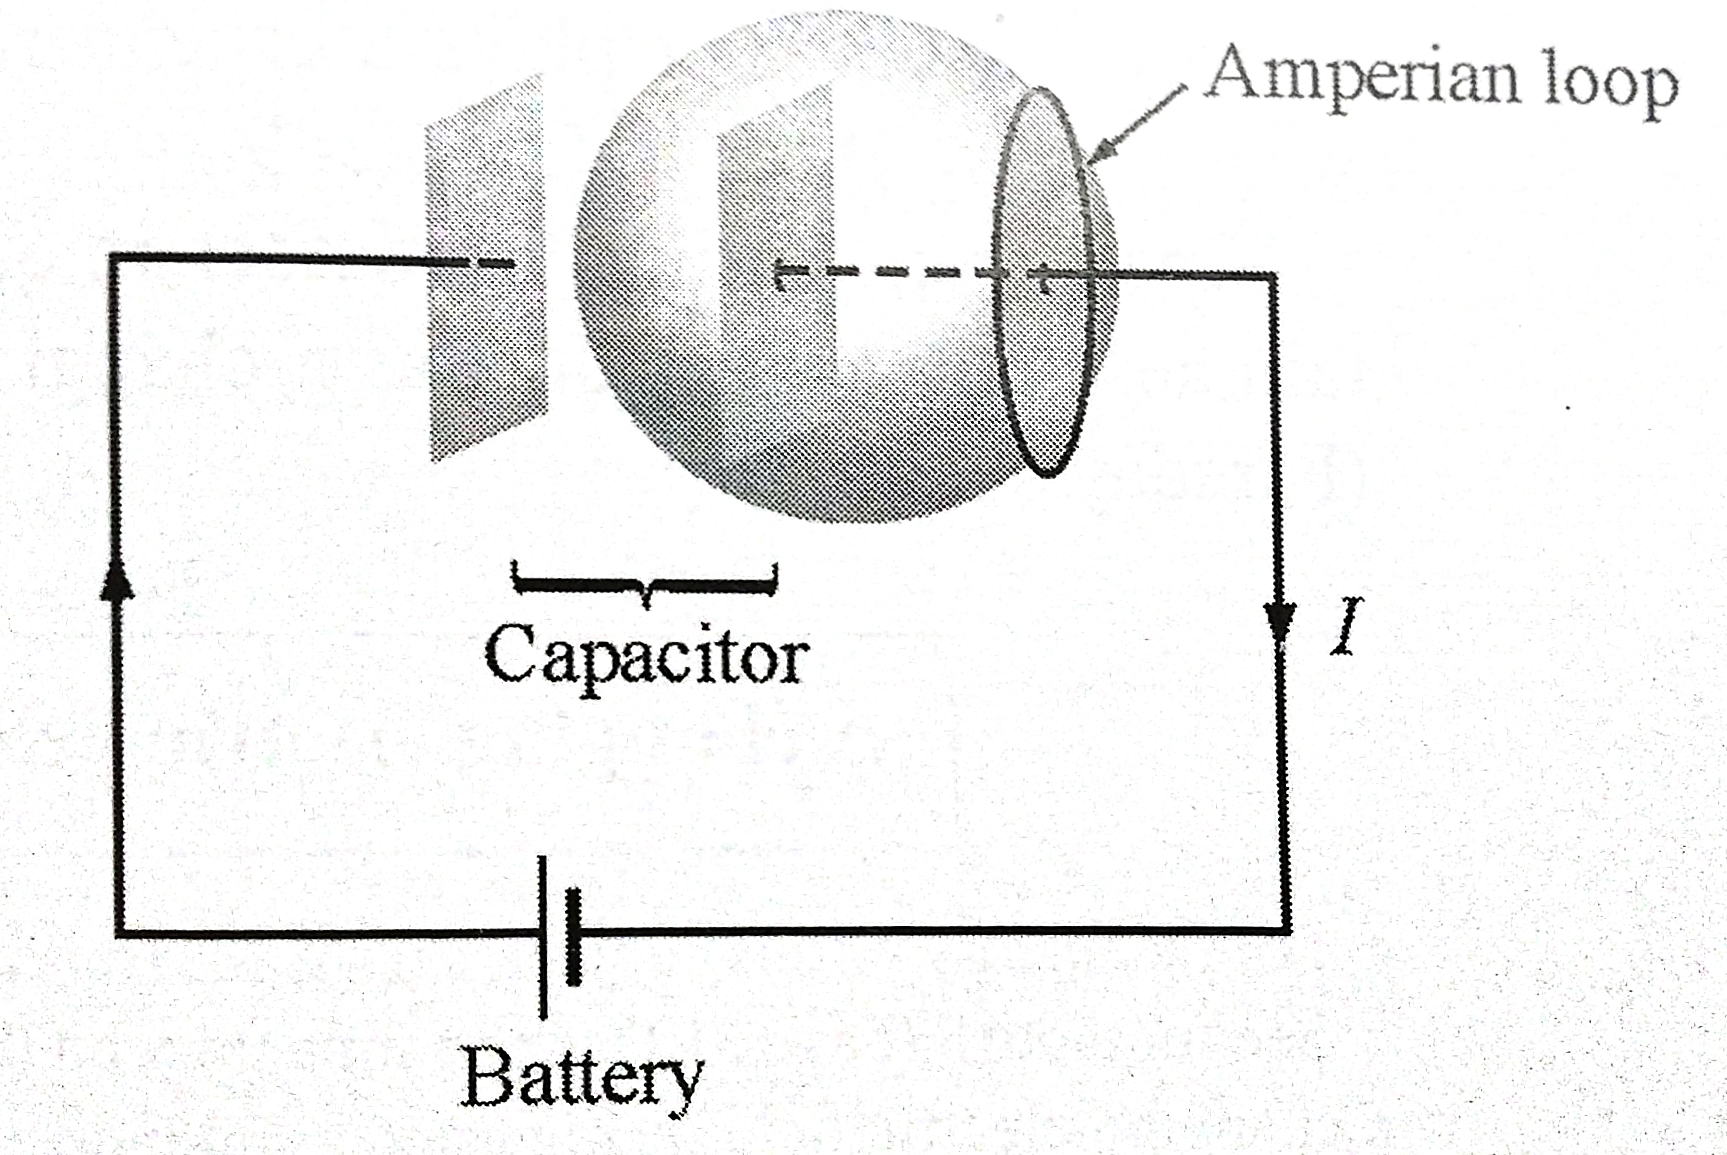
\includegraphics[width=7cm] {img/charging}
	\end{figure}
	
	For the Amperian loop draw in the diagram, the choice of surface has a significant impact on the value of $ I_\text{enc} $. For a flat disk, $ I_\text{enc}=0  $; however, we can just as well define a ``balloon" surface that circumvents the current such that $ I_\text{enc} =0 $. This is clearly a contradiction.
	
	These issues can be fixed mathematically. Suppose there exists some $ \bd{x} $ such that,
	\begin{equation}
		\curl \B = \mu_0 \bd{J} + \bd{x}
	\end{equation}
	Then,
	\begin{align}
		\div \left(\curl \B\right) &= \mu_0\div\bd{J} + \div\bd{x}\\
		&= \mu_0\left(-\pdv{\rho}{t}\right) + \div\bd{x}\\
		&= -\mu_0\left[\pdv{}{t}\left(\epsilon_0\div\E\right)\right]+ \div\bd{x}\\
		&= \div \left( -\mu_0\epsilon_0\pdv{\E}{t} + \bd{x}\right) = 0
	\end{align}
	Thus,
	\begin{equation}
		\curl \B = \mu_0 \bd{J} + \mu_0\epsilon_0\pdv{\E}{t}
	\end{equation}
	We can define the displacement current,
	\begin{equation}
		\boxed{\bd{J}_d \equiv \epsilon_0\pdv{\E}{t}}
	\end{equation}
	such that,
	\begin{equation}
		\boxed{\curl \B = \mu_0 \left(\bd{J} + \bd{J}_d\right)}
	\end{equation}
	
	Thus, we see that a changing electric field induces a magnetic field. This is known as Faraday's law. The displacement current is experimentally challenging to measure and was really confirmed with Hertz's experiments on electromagnetic waves.
	
	\section{Maxwell's Equations}
	We have compiled the governing equations for electrodynamics,
	\begin{empheq}[box=\fbox]{align}
		\begin{aligned}
			&\div \E = \frac{1}{\epsilon_0}\rho \qquad&&\text{(Gauss's law)}\\
			&\div \B= 0\\
			&\curl \E = -\pdv{\B}{t} \qquad&&\text{(Faraday's law)}\\
			&\curl \B = \mu_0\b{J} + \mu_0\epsilon_0\pdv{\E}{t} \qquad&&\text{(Amp\`ere's law with}\\
			& \qquad && \text{Maxwell's correction)}
		\end{aligned}
	\end{empheq}
	
	Notice that the asymmetry of Maxwell's equations results from the fact that, as far as we can tell, there is no magnetic charge: $ \rho_m = 0 $.

	\section{Maxwell's Equations in Matter}
	Often times, it is convenient to write Maxwell's equation in terms of the variables for polarized matter. The total charge density can be written as,
	\begin{align}
		\rho &= \rho_f + \rho_b \\
		&= \rho_f - \div\P
	\end{align}
	In the electrodynamic case, there is an additional polarization current, $ \bd{J_p} = \partial\P/\partial t $, that results from changes in the electric polarization\footnote{Imagine a chunk of matter with increasing polarization. As the polarization increases, the charge accumulation on both ends also increases, resulting in a current.},
	\begin{align}
		\bd{J} &= \bd{J}_f + \bd{J}_b + \bd{J}_p \\
		&= \bd{J}_f + \curl{\M} + \pdv{\P}{t}
	\end{align}
	We can rewrite Gauss' law,
	\begin{equation}
		\div\E = \frac{1}{\epsilon_0}\left(\rho_f - \div\P\right)
	\end{equation}
	\begin{equation}
		\div \left(\epsilon_0\E + \P\right) = \rho_f
	\end{equation}
	\begin{equation}
		\div\D = \rho_f
	\end{equation}
	Rewriting Amp\`ere's law,
	\begin{equation}
		\curl\B = \mu_0 \left(\bd{J}_f + \curl{\M} + \pdv{\P}{t}\right) + \mu_0\epsilon_0\pdv{\E}{t}
	\end{equation}
	\begin{equation}
		\curl{\left(\frac{1}{\mu_0}\B - \M\right)} = \bd{J}_f + \pdv{}{t}\left(\epsilon_0\E +\P\right)
	\end{equation}
	\begin{equation}
		\curl\H =\bd{J}_f + \pdv{\D}{t}
	\end{equation}
	
	Thus, Maxwell's equation in matter written in terms of free changes and currents,
	\begin{empheq}[box=\fbox]{align}
		\begin{aligned}
			&\div\D = \rho_f\qquad&
			&\div \B= 0
			\\
			&\curl \E = -\pdv{\B}{t} \qquad&
			&\curl\H =\bd{J}_f + \pdv{\D}{t} 
		\end{aligned}
	\end{empheq}
	
	Notice that $ \partial\D/\partial t $ plays the role of the displacement current in this case---hence $ \D $ is the ``displacement" field.
	
	\bibliographystyle{ieeetr}
	\bibliography{ref.bib}
	\nocite{*}
	
	\appendix
	\chapter{Field and Source Points}
	
	Within some charge distribution, $ \boldsymbol{r' }$ denotes a source point and $ \boldsymbol{r }$ denotes the field point---the point of interest. We define the cursive $ \brcurs $ as the displacement of the field point relative to the source point,
	\begin{equation}
		\boxed{\brcurs \equiv \boldsymbol{r}-\boldsymbol{r'}}
	\end{equation}
	\begin{figure}[H]
		\centering
		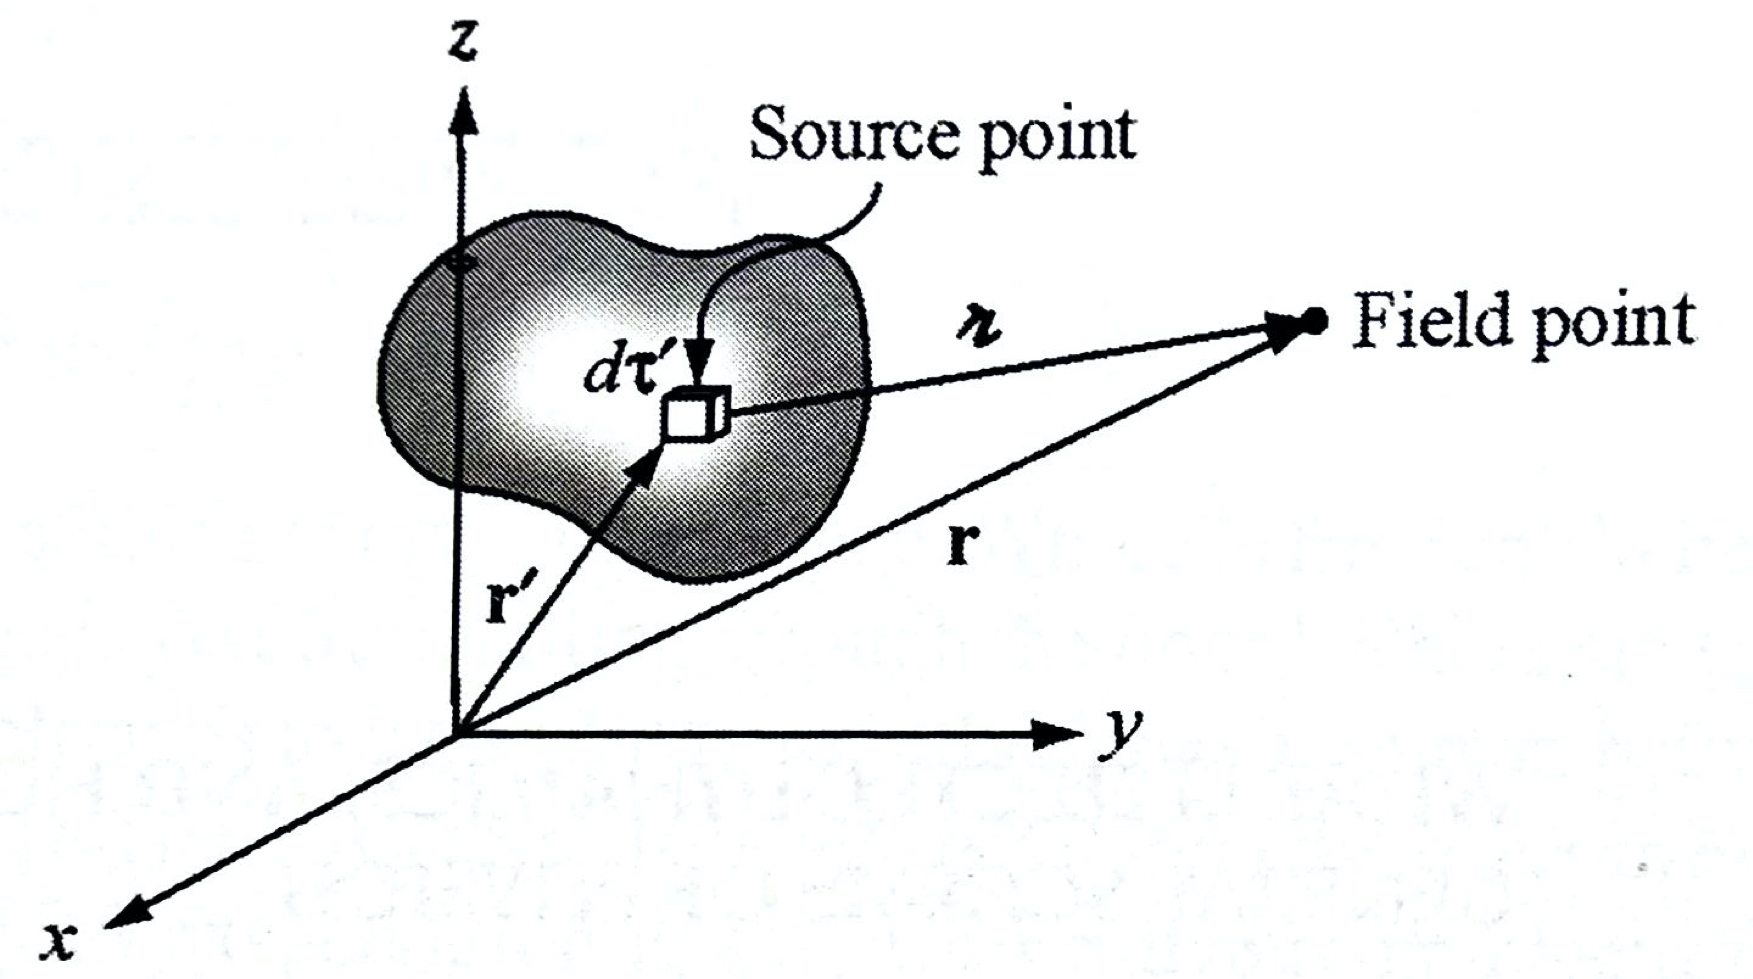
\includegraphics[width=8.5cm] {img/rs}
	\end{figure}
	
	\chapter{Calculus Aside I}
	
	Here we are concerned with finding the divergence of the field $ \boldsymbol{v}(\boldsymbol{r}) = \boldsymbol{\hat{r}}/r^2$. Recall that in spherical coordinates, the divergence becomes,
	\begin{equation}
		\div \boldsymbol{A} = \frac{1}{r^2}\pdv{}{r}\left(r^2A_r\right) + \frac{1}{r\sin\theta}\pdv{}{\theta}\left(A_\theta\sin\theta\right) + \frac{1}{r\sin\theta}\pdv{A_\phi}{\phi}
	\end{equation}
	Thus,
	\begin{equation}
		\div \boldsymbol{v} = \frac{1}{r^2}\pdv{}{r}\left(r^2 \frac{1}{r^2}\right) = 0
	\end{equation}
	This implies that the divergence is zero for all space. While this seems reasonable for $ r\neq 0 $, we see from the field diagram below that the origin is not divergence-less. There is a contradiction.
	\begin{figure}[H]
		\centering
		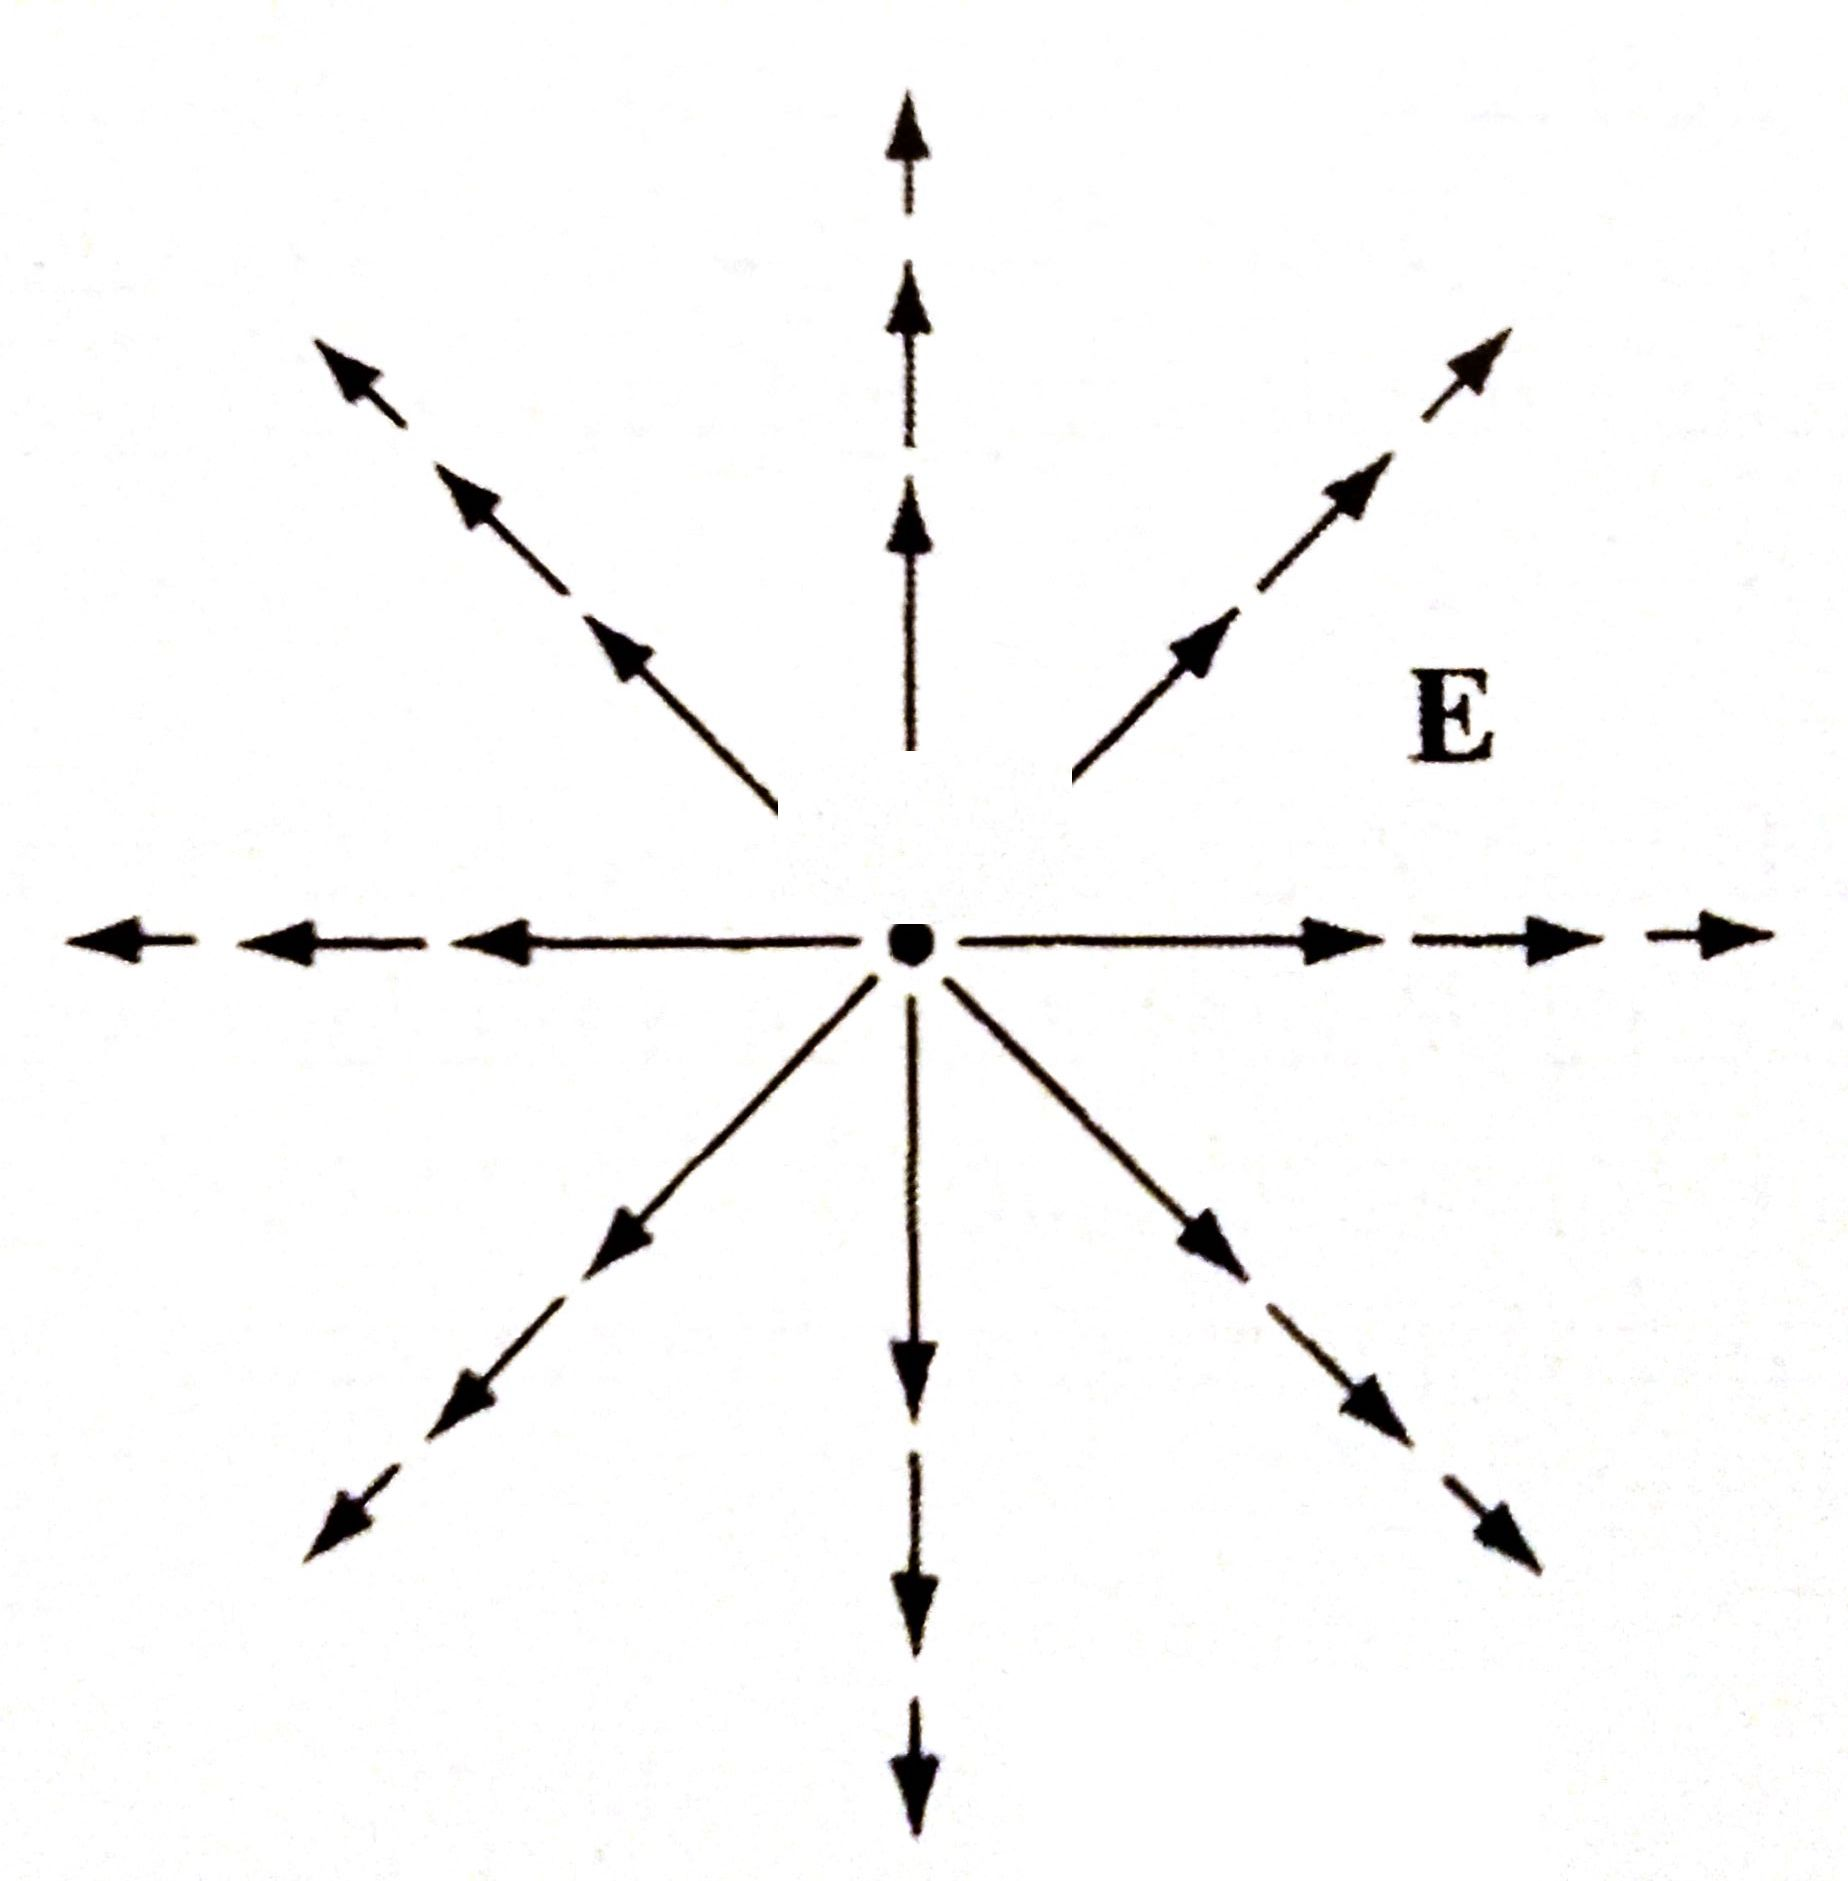
\includegraphics[width=4.5cm] {img/e_field}
	\end{figure}
	
	The cause of this contradiction is that as $ r $ tends to zero, the electric field blows up---the field is discontinuous at the origin. So what does this mean for the divergence? To answer this question, let's examine the Divergence Theorem in a spherical region of radius $ R $ centered on the origin, {\color{red}\uppercase{why is this valid, the div thm is only defined for continuous functions}}
	\begin{align}
		\int_V \left(\div \boldsymbol{v}\right)\,d\tau &= \oint_S \boldsymbol{v}\cdot d\boldsymbol{a}\\
		&= \oint_S \left(\frac{1}{R^2}\boldsymbol{\hat{r}}\right)\cdot\left(R^2\sin\theta\,d\theta\, d\phi \,\boldsymbol{\hat{r}}\right)\\
		&= \left(\int_0^\pi \sin\theta\,d\theta\right)\left(\int_0^{2\pi} d\phi\right) = 2\cdot 2\pi = 4\pi
	\end{align}
	
	The value of the integral is independent of $ R $, so it must hold that the divergence is zero everywhere outside the origin. Thus, the entire value of the integral must be a result of the divergence at the origin. In other words,
	\begin{equation}
		\div \left(\frac{\boldsymbol{\hat{r}}}{r^2}\right) = 4\pi\,\delta(\boldsymbol{r})
	\end{equation}
	where $ \delta(\boldsymbol{r}) $ is the three-dimensional Dirac delta function. Note that we use the $ \grad $ symbol to represent the derivative with respect to $ \boldsymbol{r} $ and $ \grad' $ to represent the derivative with respect to $ \boldsymbol{r}' $. With this in mind, it follows that,
	\begin{equation}
		\boxed{\div \left(\frac{\hrcurs}{\rcurs^2}\right) = 4\pi\,\delta(\boldsymbol{\brcurs})}
	\end{equation}
	
	Recall that $ \brcurs = \boldsymbol{r} - \boldsymbol{r'} $ and that $ \boldsymbol{r'} $ is held constant as we take the derivative with respect of $ \boldsymbol{r }$. Finally, we point out another fun fact,
	\begin{equation}
		\grad\left(\frac{1}{r}\right) = -\frac{\boldsymbol{\hat{r}}}{r^2}
	\end{equation}
	so, 
	\begin{equation}
		\laplacian\left(\frac{1}{r}\right) = -4\pi\,\delta(\boldsymbol{r})
	\end{equation}
	
	\chapter{Calculus Aside II}\label{appendix:aside2}
	
	While certainly not a very challenging calculation, $ \grad'\left(1/\rcurs\right)  $ must be treated with care,
	\begin{align}
		\grad'\left(\frac{1}{\rcurs}\right) &= \frac{\partial}{\partial x'}{\color{blue} \left[(x-x')^2 + (y-y')^2 + (z-z')^2\right]}^{-1/2}\unit{x} + \frac{\partial}{\partial y'} {\color{blue} \left(\right)}^{-1/2}\unit{y} + \frac{\partial}{\partial z'} {\color{blue} \left(\right)}^{-1/2}\unit{z}\\
		&= -\frac{1}{2}{\color{blue} \left(\right)}^{-3/2}\left[-2(x-x')\unit{x}\right]-\frac{1}{2}{\color{blue} \left(\right)}^{-3/2}\left[-2(y-y')\unit{y}\right]-\frac{1}{2}{\color{blue} \left(\right)}^{-3/2}\left[-2(z-z')\unit{z}\right]\\
		&= {\color{blue} \left(\right)}^{-3/2} \left[(x-x')\unit{x} + (y-y')\unit{y} + (z-z')\unit{z}  \right]\\
		&= \frac{\brcurs}{\rcurs^3} = \frac{\hrcurs}{\rcurs^2}
	\end{align}
	\begin{equation}
		\boxed{\grad'\left(\frac{1}{\rcurs}\right) =\frac{\hrcurs}{\rcurs^2}}
	\end{equation}
	
\end{document}